\documentclass{article}
\title{The Arf Invariant}
\author{Alwyn Bakker}


\usepackage{caption, subcaption, amsmath, amssymb, amsthm, tikz}
\usepackage{color}
\usetikzlibrary{arrows, decorations.markings}
\begin{document}
%tikz setup
	%sets up style for arrows partway along lines
	\tikzset{->-/.style={decoration={markings, mark=at position #1 with {\arrow[scale=1.5]{>}}}, postaction={decorate}}} 
	\tikzset{-<-/.style={decoration={markings, mark=at position #1 with {\arrow[scale=1.5]{<}}}, postaction={decorate}}}

%amsthm setup
	%sets up definition style
	\theoremstyle{definition}
	\newtheorem{definition}{Definition}[section]
	
	%sets up theorem style
	\newtheorem{theorem}{Theorem}[section]

\maketitle

\section{Knots}

%%----------------------------------------------------Equivalent Knots Figure---------------------------------------------------------------------%%
\begin{figure}
	\begin{subfigure}[t]{0.5\linewidth}
	\centering
	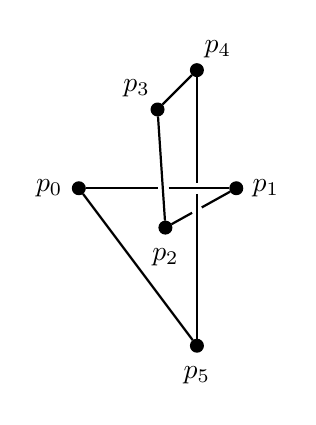
\begin{tikzpicture}
	\tikzstyle{every node} = [draw, thick, circle, fill=black, inner sep=1.5pt]
	\node [label=left:{$p_0$}] (p0) at (0,0) {}; \node[label=right:{$p_1$}] (p1) at (2,0) {}; \node[label=below:{$p_2$}] (p2) at (1.1,-0.5) {}; \node[label=above left:{$p_3$}] (p3) at (1,1) {}; \node [label=above right:{$p_4$}] (p4) at (1.5,1.5) {}; \node[label=below:{$p_5$}] (p5) at (1.5,-2) {};
	
	\draw[thick] (p0) -- (1,0); \draw[thick, shorten <=4] (1,0) -- (p1); \draw[thick, shorten >=2] (p1) -- (1.5,-2.5/9); \draw[thick, shorten <=2] (1.5,-2.5/9) -- (p2); \draw[thick] (p2) -- (p3); \draw[thick] (p3) -- (p4); \draw [thick, shorten >=2] (p4) -- (1.5, 0); \draw[thick, shorten <=2] (1.5,0) -- (p5); \draw[thick] (p5) -- (p0);
	\end{tikzpicture}
	\caption{Knot A}
	\label{fig:equivalent knots a}
	\end{subfigure}
	~
	\begin{subfigure}[t]{0.5\linewidth}
	\centering
	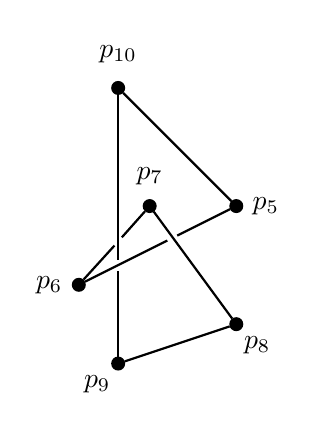
\begin{tikzpicture}
	\tikzstyle{every node} = [draw, thick, circle, fill=black, inner sep=1.5pt]
	\node [label=right:{$p_5$}] (p5) at (0,0.5) {}; \node[label=left:{$p_6$}] (p6) at (-2,-0.5) {}; \node[label=above:{$p_7$}] (p7) at (-1.1,0.5) {}; \node[label=below right:{$p_8$}] (p8) at (0,-1) {}; \node [label=below left:{$p_9$}] (p9) at (-1.5,-1.5) {}; \node[label=above:{$p_{10}$}] (p10) at (-1.5,2) {};
	
	\draw[thick] (p5) -- (-0.75,0.125); \draw[thick, shorten <=4] (-0.75,0.125) -- (p6); \draw[thick, shorten >=2] (p6) -- (-1.5,0.05); \draw[thick, shorten <=2] (-1.5,0.05) -- (p7); \draw[thick] (p7) -- (p8); \draw[thick] (p8) -- (p9); \draw [thick, shorten >=2] (p9) -- (-1.5, -.25); \draw[thick, shorten <=2] (-1.5,-.25) -- (p10); \draw[thick] (p10) -- (p5);
	\end{tikzpicture}
	\caption{Knot B}
	\end{subfigure}
\caption{Two distinct, ordered sets of points that give us equivalent trefoil knots.}
\label{fig:equivalent knots}
\end{figure}

%%----------------------------------------------------Inquivalent Knots Figure--------------------------------------------------------------------%%
\begin{figure}
	\begin{subfigure}[t]{0.5\linewidth}
	\centering
	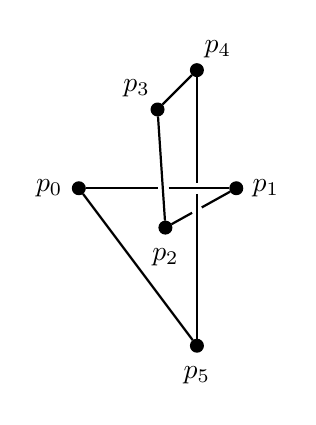
\begin{tikzpicture}
	\tikzstyle{every node} = [draw, thick, circle, fill=black, inner sep=1.5pt]
	\node [label=left:{$p_0$}] (p0) at (0,0) {}; \node[label=right:{$p_1$}] (p1) at (2,0) {}; \node[label=below:{$p_2$}] (p2) at (1.1,-0.5) {}; \node[label=above left:{$p_3$}] (p3) at (1,1) {}; \node [label=above right:{$p_4$}] (p4) at (1.5,1.5) {}; \node[label=below:{$p_5$}] (p5) at (1.5,-2) {};
	
	\draw[thick] (p0) -- (1,0); \draw[thick, shorten <=4] (1,0) -- (p1); \draw[thick, shorten >=2] (p1) -- (1.5,-2.5/9); \draw[thick, shorten <=2] (1.5,-2.5/9) -- (p2); \draw[thick] (p2) -- (p3); \draw[thick] (p3) -- (p4); \draw [thick, shorten >=2] (p4) -- (1.5, 0); \draw[thick, shorten <=2] (1.5,0) -- (p5); \draw[thick] (p5) -- (p0);
	\end{tikzpicture}
	\caption{Knot A: Trefoil Knot}
	\end{subfigure}
	~
	\begin{subfigure}[t]{0.5\linewidth}
	\centering
	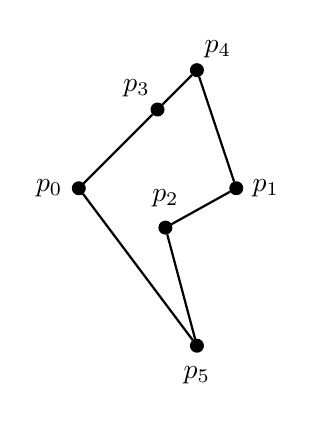
\begin{tikzpicture}
	\tikzstyle{every node} = [draw, thick, circle, fill=black, inner sep=1.5pt]
	\node [label=left:{$p_0$}] (p0) at (0,0) {}; \node[label=right:{$p_1$}] (p1) at (2,0) {}; \node[label=above:{$p_2$}] (p2) at (1.1,-0.5) {}; \node[label=above left:{$p_3$}] (p3) at (1,1) {}; \node [label=above right:{$p_4$}] (p4) at (1.5,1.5) {}; \node[label=below:{$p_5$}] (p5) at (1.5,-2) {};
	\draw[thick] (p0) -- (p3) -- (p4) -- (p1) -- (p2) -- (p5) -- (p0);
	\end{tikzpicture}
	\caption{Knot B: Unknot}
	\end{subfigure}
\caption{One set of distinct points gives two different knots when joined in a different order.}
\label{fig:inequivalent knots}
\end{figure}


%%-----------------------------------------------------Knot Definition-------------------------------------------------------------------------%%

\begin{definition}[Knot]
A knot is a simple closed polygonal curve in $\mathbb{R}^3$. %\cite[Liv93]
\end{definition}
A polygonal curve is created by `joining the dots'. We pick an ordered set of distinct points $(p_0,p_1,...,p_n) \in \mathbb{R}^3$, and define $[p_i,p_j]$ to be the line segment joining points $p_i$, $p_j$. The polygonal curve is $\cup _{i=0}^n [p_i, p_{i+1}]$, with $p_{n+1}=p_0$.\\

This tends to result in very jagged-looking knots, so it is more usual to represent a knot as a smooth curve (i.e. the number of distinct points in our set tends to infinity).\\

Note that carefully selecting two different sets of distinct points can give us knots that are equivalent, as in Fig (\ref{fig:equivalent knots}); Knot A can be transformed into Knot B by a half-circle rotation and slightly translating individual points within the line boundaries. Additionally, linking one set of distinct points in two different orders can give us inequivalent knots, as in Fig (\ref{fig:inequivalent knots}). As our sets of points become larger, it can be very difficult to determine if two knots are equivalent, especially if we need to `untangle' them first. (In fact, it is already very difficult to prove that the examples we have provided are equivalent or inequivalent!) This means we need to develop tools to help us distinguish between inequivalent knots. These commonly take the form of \emph{invariants}, knot properties that remain consistent regardless of any deformations the knot might undergo. One such invariant is the Arf invariant, which is the subject of this report.\\
\\
In order to define `untangling' a knot, it can be useful to think of it as a one dimensional manifold, and `untangling' as a kind of mapping between 1-manifolds.\\

\begin{definition}[] An $n$-dimensional \textbf{manifold} is a topological space where every point in the space has a neighbourhood that is homeomorphic to $\mathbb{R}^n$. In our case, $n=1$, so each point on the knot must have a neighbourhood homeomorphic to $\mathbb{R}$.\\
\end{definition}



%%-------------------------------------------------Isotopy Definition-------------------------------------------------------------------------------%%
\begin{definition}[] An \textbf{isotopy} is a continuous transformation from one embedding of a manifold $M$ in a space $N$ to another embedding of $M$ in $N$ in such a way that at every point in time along the transformation it is still an embedding in $N$. More precisely, an isotopy is a continuous function $H: M\times I \rightarrow N$, where $I=[0,1]$, such that $H_t:M\rightarrow N$, defined by $H_t(x)=H(t,x)$ is an embedding for all $t$, and $H_0=f_0$, $H_1=f_1$.
\end{definition}
This would appear to be a good definition for `untangling' a knot, but it is not quite rigorous enough yet. Under this interpretation, shrinking part of a knot to a point would be a permissible way to untangle it, rendering all knots isotopically equivalent to the unknot. We need to narrow the definition to close this loophole.\\

%%-------------------------------------------------Ambient Isotopy Definition---------------------------------------------------------------------%%
\begin{definition}[] An \textbf{ambient isotopy} is like an isotopy, with the caveat that it is the space \emph{containing} the embedding of the manifold $M$ that is being continously transformed rather than $M$ itself. The embedding is essentially being carried along with the transformation of the space. For our purposes, the ambient space is $\mathbb{R}^3$.
\end{definition}
This tweak to the definition of `untangling' prevents us from shrinking part of a knot to a point, as that would `break' the space around the knot.\\

%%-------------------------------------------------Knot Diagrams Text---------------------------------------------------------------------%%
However, we're not quite done. In order to compare embeddings, we need some way to represent them in two dimensions, without losing any information about under- and over-crossings. The solution to this is the \textbf{knot diagram}. We project the knot onto a plane, then introduce a convention for recording crossing information; sections of the knot that go under other sections have a visible break at the crossing, as in Fig (\ref{fig:equivalent knots a}), where the section from $p_4$ to $p_5$ crosses under the section from $p_0$ to $p_1$ but over the section from $p_1$ to $p_2$. We also require that all crossings are at \textbf{double points}, where only two sections cross each other, and are \textbf{transverse}, where each section is bisected by the crossing. If we permit crossings that are not at transverse double points, we lose important information. At a transverse double point such as in Fig (\ref{fig:knot diagrams a}) it is easy to tell which strand is on top, but at a transverse triple point like Fig (\ref{fig:knot diagrams b}) we have lost information about overlapping and connections; we cannot tell whether the section from $a$ to $d$ is above or below the section from $b$ to $c$, or even whether $a$ connects to $c$ or $d$. Likewise, a non-transverse double point such as in Fig (\ref{fig:knot diagrams c}) is also lacking information; we cannot tell how the section beginning at $e$ connects to any of the other sections, or whether it is above or below the strand composed of the two sections it does not connect to.\\
%%-------------------------------------------------Regular Projection Definition------------------------------------------------------------------%%
\begin{definition}[] A knot projection is \textbf{regular} if it is injective everywhere except at a finite number of crossing points, which must be exclusively transverse double points. \textcolor{red}{Every knot has a regular projection, because any projection of a knot can be perturbed to a regular projection.}\\
\end{definition}

Now that we have a way of diagramming a knot embedding, we can discuss some techniques for showing embeddings are equivalent.\\


%%-------------------------------------------------Knot Diagrams Figure---------------------------------------------------------------------%%

\begin{figure}
\centering
	\begin{subfigure}[b]{0.3\linewidth}
	\centering
	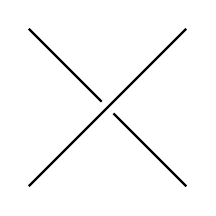
\begin{tikzpicture}
	\draw [thick] (-1,-1) to (1,1); \draw [thick, shorten >=3] (1,-1) to (0,0); \draw [thick, shorten <=3] (0,0) to (-1,1);
	\end{tikzpicture}
	\caption{Transverse double point.}
	\label{fig:knot diagrams a}
	\end{subfigure}\hfill%
	\begin{subfigure}[b]{0.3\linewidth}
	\centering
	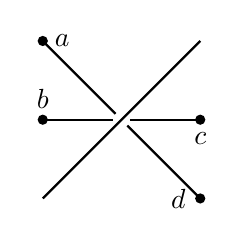
\begin{tikzpicture}
	\tikzstyle{every node} = [draw, thick, circle, fill=black, inner sep=1pt]
	\node[label=right:{$a$}] at (-1, 1) {}; \node[label=above:{$b$}] at (-1,0) {}; \node[label=below:{$c$}] at (1,0) {}; \node[label=left:{$d$}] at (1,-1) {};
	\draw [thick] (-1,-1) to (1,1); \draw [thick, shorten >=3] (1,-1) to (0,0); \draw [thick, shorten <=3] (0,0) to (-1,1); \draw[thick, shorten >=3] (-1,0) to (0,0); \draw[thick, shorten <=3] (0,0) to (1,0);
	\end{tikzpicture}
	\caption{Transverse triple point.}
	\label{fig:knot diagrams b}
	\end{subfigure}\hfill%
	\begin{subfigure}[b]{0.3\linewidth}
	\centering
	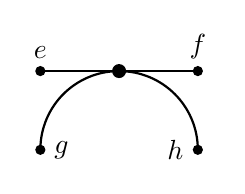
\begin{tikzpicture}
	\tikzstyle{every node} = [draw, thick, circle, fill=black, inner sep=1pt]
	\node[label=above:{$e$}] at (-1,0) {}; \node[label=above:{$f$}] at (1,0) {}; \node[label=right:{$g$}] at (-1,-1) {}; \node[label=left:{$h$}] at (1,-1) {}; 
	\draw[thick] (-1,0) to (1,0); \draw[thick] (-1,-1) to [out=90, in=180] (0,0) to [out=0, in=90] (1,-1);
	\tikzstyle{every node} = [draw, thick, circle, fill=black, inner sep=1.5pt]
	\node at (0,0) {};
	\end{tikzpicture}
	\caption{Non-transverse double point.}
	\label{fig:knot diagrams c}
	\end{subfigure}%
\caption{Only (a) is permitted in a knot diagram; (b) and (c) do not contain enough information to indicate which section crosses over which.}
\label{fig:knot diagrams}
\end{figure}


%%-------------------------------------------------------Reidemeister Moves Figure-------------------------------------------------------------%%

\begin{figure}
\centering
	\begin{subfigure}[b]{0.3\linewidth}
	\centering
		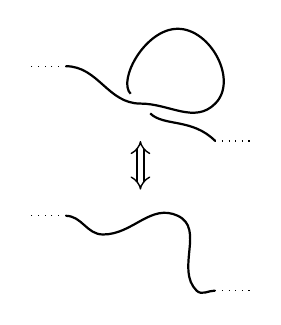
\begin{tikzpicture}[>=implies, scale=0.95]
		%top
		\draw [thick, shorten >=5] (-1,0.5) to [out=0,in=180] (0,0) to [out=0, in=-135] (1,0) to [out=45, in=0] (0.5, 1) to [out=180, in=135] (0,0);
		\draw [thick, shorten <=5] (0,0) to [out=-45, in=135] (1,-0.5);
		%bottom
		\draw [thick] (-1,-1.5) to [out=0, in=180] (-0.5,-1.75) to [out=0, in=155] (0.5,-1.5) to [out=-25, in=135] (0.75,-2.5) to [out=-45, in=180] (1,-2.5);
		%arrow
		\draw [line width=0.5pt, double distance=2pt, <->] (0,-0.5) to [out=-90, in=90] (0,-1.15);
		%extra knot bits
		\draw[dotted] (-1,0.5) -- (-1.5,0.5); \draw[dotted] (1,-0.5) -- (1.5, -0.5);
		\draw[dotted] (-1,-1.5) -- (-1.5,-1.5); \draw[dotted] (1,-2.5) -- (1.5, -2.5);
		\end{tikzpicture}
	\caption{Type 1: Untwisting a loop.}
	\end{subfigure}\hfill
	~
	\begin{subfigure}[b]{0.3\linewidth}
	\centering
		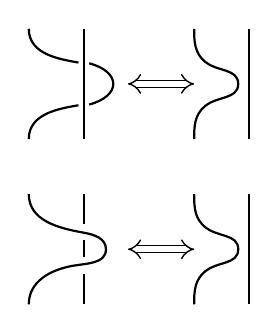
\begin{tikzpicture}[>=implies, scale=1.4]
		%top
			%left side
			\draw [thick] (0,0.5) to (0,-0.5);
			\draw [thick, shorten >=2] (-0.5,0.5) to [out=-90, in=170] (0,0.185);
			\draw [thick, shorten >=2, shorten <=2, distance=10] (0,0.2) to [out=-15, in=15] (0,-0.2);
			\draw [thick, shorten <=2] (0,-0.185) to [out=-170, in=90] (-0.5,-0.5);
			% right side
			\draw [thick] (1.5,0.5) to (1.5,-0.5);
			\draw [thick] (1,0.5) to [out=-90, in=140] (1.1,0.2) to [out=-40, in=90] (1.4,0) to [out=-90, in=40] (1.1,-0.2) to [out=-140,in=90] (1,-0.5);
			%arrow
			\draw [line width=0.5pt, double distance=2pt, <->] (0.4,0) to (1,0);
		%bottom
			%left side
			\draw [thick] (-0.5,-1) to [out=-90, in=170] (0,-1.35) to [out=-10, in=90] (0.2,-1.5) to [out=-90, in=10] (-0.1,-1.65) to [out=-170,in=90] (-0.5,-2);
			\draw [thick] (0,-1) to (0,-1.27);
			\draw [thick] (0,-1.42) to (0,-1.57);
			\draw [thick] (0,-1.72) to (0,-2);
			%right side
			\draw [thick] (1,-1) to [out=-90, in=140] (1.1,-1.3) to [out=-40, in=90] (1.4,-1.5) to [out=-90, in=40] (1.1,-1.7) to [out=-140,in=90] (1,-2);
			\draw [thick] (1.5,-1) to (1.5,-2);
			%arrow
			\draw [line width=0.5pt, double distance=2pt, <->] (0.4,-1.5) to (1,-1.5);
		\end{tikzpicture}
	\caption{Type 2: Moving one strand over another.}
	\end{subfigure}\hfill
	~
	\begin{subfigure}[b]{0.3\linewidth}
	\centering
		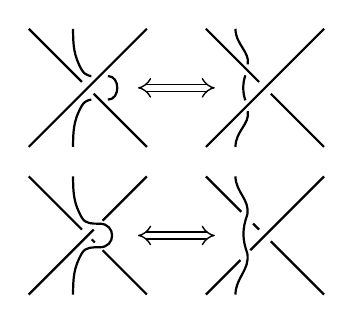
\begin{tikzpicture}[>=implies, scale=0.75]
		%top
			%left side
			\draw [thick] (1,1) to (-1,-1);
			\draw [thick, shorten >=3] (-1,1) to (0,0);
			\draw [thick, shorten <=3] (0,0) to (1,-1);
			\draw [thick, shorten >=3] (-0.25,1) to [out=-90, in=120] (-0.1,0.3) to [out=-60, in=180] (0.2,0.2);
			\draw [thick, shorten <=3, shorten >=3, distance=10] (0.2,0.2) to [out=0, in=0] (0.2,-0.2);
			\draw [thick, shorten <=3] (0.2,-0.2) to [out=180, in=60] (-0.1,-0.3) to [out=-120, in=90] (-0.25,-1);
			%right side
			\draw [thick] (4,1) to (2,-1);
			\draw [thick, shorten >=3] (2,1) to (3,0);
			\draw [thick, shorten <=3] (3,0) to (4,-1);
			\draw [thick, shorten >=1] (2.5,1) to [out=-90, in=80] (2.7,0.35);
			\draw [thick, shorten <=2, shorten >=2] (2.7, 0.3) to [out=-110, in=110] (2.7,-0.3);
			\draw [thick, shorten <=1] (2.7, -0.35) to [out=-80, in=90] (2.5,-1);
			%arrow
			\draw [line width=0.5pt, double distance=2pt, <->] (0.85,0) to (2.15,0);
		%bottom
			%left side
			\draw [thick] (-0.25,-1.5) to [out=-90, in=120] (-0.1,-2.2) to [out=-60, in=180] (0.2,-2.3) to [out=0, in=0, distance=8] (0.2,-2.7) to [out=180, in=60] (-0.1,-2.8) to [out=-120, in=90] (-0.25,-3.5);
			\draw [thick] (1,-1.5) to (0.25,-2.25);
			\draw [thick] (0.1,-2.4) to (-1,-3.5);
			\draw [thick, shorten >=3] (-1,-1.5) to (0,-2.5);
			\draw [thick, shorten <=2] (0,-2.5) to (0.12,-2.62);
			\draw [thick] (0.25,-2.75) to (1,-3.5);
			%right side
			\draw [thick] (2.5,-1.5) to [out=-90, in=80] (2.7,0.-2.15) to [out=-110, in=110] (2.7,-2.8) to [out=-80, in=90] (2.5,-3.5);
			\draw [thick] (2,-1.5) to (2.6, -2.1);
			\draw [thick, shorten <=6, shorten >=3] (2.6, -2.1) to (3,-2.5);
			\draw [thick, shorten <=3] (3,-2.5) to (4,-3.5);
			\draw [thick] (4,-1.5) to (2.75, -2.75);
			\draw [thick, shorten <=5] (2.75,-2.75) to (2,-3.5);
			%arrow
			\draw [line width=0.5pt, double distance=2pt, <->] (0.85,-2.5) to (2.15,-2.5);
		\end{tikzpicture}
	\caption{Type 3: Moving a strand past a crossing.}
	\end{subfigure}
\caption{The three Reidemeister moves.}
\label{fig:reidemeister moves}
\end{figure}

%%--------------------------------------------------Reidemeister Moves Text---------------------------------------------------------------------%%
Two embeddings that are equivalent up to ambient isotopy are considered to be the same knot. In order to show that two embeddings are equivalent we demonstrate that there is a sequence of `rearrangements' that will allow us to transform the knot from one embedding to the other by an ambient isotopy. These rearrangements are known as the \emph{Reidemeister moves.}\\

\begin{definition}[] A \textbf{Reidemeister move} permits us to move between one diagram shown in Fig (\ref{fig:reidemeister moves}) and its accompanying diagram. The before and after diagrams are of the same knot, and the part of the knot outside the diagram is unchanged. Type 1 Reidemeister moves allow us to twist or untwist a loop. Type 2 moves allow us to move a section of one strand over another. Type 3 moves allow us to move a section of one strand over the crossing of another two.\\
\end{definition}

\begin{theorem}Two knot diagrams are equivalent if and only if there is a sequence of Reidemeister moves and planar isotropies that transforms one to the other.\\
\end{theorem}
The `if' part of this theorem is intuitively obvious; since performing any of the Reidemeister moves on a knot diagram does not change the initial knot, the diagram that results from applying any number of the moves must be of the same knot we started with. However, the sufficiency of the Reidemeister moves in demonstrating equivalence is less obvious. We know that we cannot change our embedding of interest into the embedding of a different knot by using Reidemeister moves. This means any rearrangement maintains the embedding, and our starting and ending knot diagrams are both of that embedding, along with any interim diagrams, meaning the Reidemeister moves are sufficient to demonstrate equivalence.\\

As useful as the Reidemeister moves are in demonstrating two knot diagrams are equivalent or inequivalent (and in the definition of invariants), it can be extremely difficult to actually find a sequence of moves that will transform one knot diagram to another, especially if one or both diagrams are complicated. Our difficulties are compounded by the fact that the upper bound to the number of Reidemeister moves that may be required to transform the initial knot diagram can be immense. For the pair of knot diagrams of the trefoil knot shown in Fig (\ref{fig:equivalent knots}), an upper bound is $2^{2^{2^{...^3}}}$, the tower of exponents being $10^{1,000,000^3}$ individual 2s tall. [from AN UPPER BOUND ON REIDEMEISTER MOVES by ALEXANDER COWARD and MARC LACKENBY, 2012] Additionally, if we are attempting to prove two knot diagrams are \emph{inequivalent} using only Reidemeister moves, we would have to check every move sequence to prove the inequivalence.\\ 
\\
 We \emph{clearly} need some other method of showing two knot diagrams are inequivalent.\\
 
 %%-----------------------------------------------------Invariant Definition-------------------------------------------------------------------------%%
\begin{definition}[Invariant] An invariant is some property of a knot that is unchanged under ambient isotopy.
\end{definition}
Depending on the invariant selected, two embeddings of a circle that share the same invariant are potentially of the same knot. (Generally, the easier an invariant is to compute, the less discriminatory it is!) However, it is more usual to attempt to prove two embeddings are not of the same knot by finding a knot invariant that gives a different result for each embedding.\\
There are many different invariants of a knot, such as the linking, knotting or bridge numbers, various polynomials, and so on. This report is primarily concerned with the Arf invariant, and the ways it can be derived or defined.\\

%%--------------------------------------------------New Section-----------------------Pass Equivalence-----------------------------------------%%

\section{The Arf Invariant Defined Via Pass-Equivalence}
\subsection{Definitions}
%%------------------------------------------------Oriented Knot Definition-------------------------------------------------------------------------%%

\begin{definition}[Orientation] An orientation can be placed on a knot embedding by choosing a direction to travel around it. In figures of knots, this is indicated by arrows on the curve, pointing in the direction of travel. A knot with an orientation is called an \textbf{oriented knot}.
\end{definition}

%%------------------------------------------------------Pass Move Definition----------------------------------------------------------------------%%
\begin{definition}[Pass Move] A pass move is a change in the embedding of an oriented knot that passes a pair of oppositely-oriented strands through a second pair of oppositely oriented strands, as in Fig (\ref{fig:pass move}).
\end{definition}
A pass-move is similar to a Reidemeister move in that it allows us to `rearrange' a knot, but unlike a Reidemeister move it is not an ambient isotopy, as it `breaks' the knot; after applying a pass-move, the knot we started with is (usually) transformed into a different knot. In addition, applying a pass-move to a knot requires the strands to be oriented; the orientation of the strands in each pair must be opposed. If we can get from one knot to another through successive pass-moves, rearranging the embedding as necessary in between each Reidemeister move, we say that the two knots are \textbf{pass equivalent}. The Arf invariant is defined in terms of pass equivalence as follows:\\

%%----------------------------------------------------Pass-Move Figure--------------------------------------------------------------------------%%

\begin{figure}
\centering
\begin{tikzpicture}
%left side
\draw [thick, ->-=0.2, ->-=0.9] (-1,1) to (1,1);
\draw [thick, -<-=0.2, -<-=0.9] (-1,0.5) to (1,0.5);
\draw [thick, ->-=0.5, shorten >=2] (-0.25,1.75) to (-0.25,1); \draw [thick, shorten <=2, shorten >=2] (-0.25,1) to (-0.25,0.5); \draw [thick, shorten <=2, ->-=0.7] (-0.25, 0.5) to (-0.25,-0.25);
\draw [thick, -<-=0.5, shorten >=2] (0.25,1.75) to (0.25,1); \draw [thick, shorten <=2, shorten >=2] (0.25,1) to (0.25,0.5); \draw [thick, shorten <=2, -<-=0.7] (0.25, 0.5) to (0.25,-0.25);
%right side
\draw [thick, ->-=0.2, ->-=0.9] (3.75, 1.75) to (3.75,-0.25);
\draw [thick, -<-=0.2, -<-=0.9] (4.25, 1.75) to (4.25,-0.25);
\draw [thick, ->-=0.5, shorten >=2] (3,1) to (3.75,1); \draw [thick, shorten <=2, shorten >=2] (3.75,1) to (4.25,1); \draw [thick, ->-=0.7, shorten <=2] (4.25,1) to (5,1);
\draw [thick, -<-=0.5, shorten >=2] (3,0.5) to (3.75,0.5); \draw [thick, shorten <=2, shorten >=2] (3.75,0.5) to (4.25,0.5); \draw [thick, -<-=0.7, shorten <=2] (4.25,0.5) to (5,0.5);
%arrow
\draw [line width =0.75pt, double distance=3pt, >=implies, <->] (1.4,0.75) to (2.6,0.75);
\end{tikzpicture}
\caption{A Pass-Move. Note that reversing the orientations of either parallel pair of lines will still give a valid pass-move.}
\label{fig:pass move}
\end{figure}

%%------------------------------------------------------Arf Invariant Definition--------------------------------------------------------------------%%
{\begin{definition}[] The \textbf{Arf invariant} $a(K)$ of a knot $K$  is defined to be $0\in \mathbb{Z}_2$ if $K$ is pass-equivalent to the unknot, and $1\in \mathbb{Z}_2$ if $K$ is pass-equivalent to the trefoil knot. 
\end{definition}

The Arf invariant is well-defined by the following theorem:

\begin{theorem}Every knot is either pass equivalent to the unknot or to the trefoil knot. Moreover, the unknot and trefoil knot are not pass equivalent to each other.\\
\end{theorem} %\cite{Ada1994}

In order to prove this, we need to explore the idea of \textbf{Seifert surfaces}.

%%------------------------------------------------Seifert Surfaces------------------------------------------------------------------------------%%

\subsection{Seifert Surfaces}
\textcolor{red}{[Definition unchanged, still needs work]}
\begin{definition}(Seifert Surface) A Seifert surface for a knot $K$ in $\mathbb{R}^3$ is a compact, oriented 2-manifold $S$ embedded in $\mathbb{R}^3$ such that the boundary of the surface $\partial S=K$, and $S$ does not have any closed surface components. cite[A SURVEY OF KNOT THEORY by AKIO KAWAUCHI]
\end{definition}
We can obtain a Seifert surface from a knot diagram with the following process. As an example, we will use the trefoil knot embedding in Fig (\ref{fig:trefoil}).
\begin{enumerate}
\item Assign an orientation to the embedding, as in Fig (\ref{fig:oriented trefoil}).
\item  Note that each crossing point in the embedding has two strands entering and two strands exiting. Connect each entering strand to the single exiting strand found to its immediate left or right.
\item We should now have a collection of oriented circles, as in Fig (\ref{fig:crossing elimination}). These are known as \textbf{Seifert circles}. If any Seifert circle is located in the interior of another Seifert circle, we move it up and out of the plane of the exterior circle. Multiple concentric Seifert circles will become `stacked', with the smallest circle at the top of the stack and the largest in the original plane, like a Tower of Hanoi.
\item Connect each Seifert circle at the old crossing points with a half-twisted band, as in Fig (\ref{fig:seifert discs}). The direction of the half-twist must mimic the original crossings; note how in Fig (\ref{fig:oriented trefoil}) the north-east strand in the top crossing swaps to the south-east, going behind the north-east to south-west strand, and in Fig (\ref{fig:seifert discs}), the top edge of the top band moves behind the bottom edge as it twists and connects to the right disc. Also note that the boundary of the surface is the oriented trefoil knot.
\end{enumerate}

 This is now a Seifert surface, but for our purpose it is useful to deform the surface further, as in Fig (\ref{fig:seifert deform 1}), with the aim of reducing the surface to a single disc with attached bands, as in Fig (\ref{fig:seifert deform 2}).

Fig (\ref{fig:seifert deform 2}) gives us a clear picture of the two half-twists in each band, but we will continue to deform until we reach a useful standard form. In general, we can replace two half-twists with a curl, as in Fig (\ref{fig:twists to curl}); we permit the left side of the strand to pass above the plane of the right, and flatten the loop back down into the plane. Applying this trick to Fig (\ref{fig:seifert deform 2}) and deforming the central disc into a `tablet' shape gives us Fig (\ref{fig:trefoil curl}).\\

Now that we have a clear picture of the trefoil knot as the boundary of a Seifert surface, we can perform the procedure with a more complicated knot and see how it compares to the trefoil `tablet'.\\

%%------------------------------------------------Trefoil Figures 1------------------------------------------------------------------------------%%
\begin{figure}
\centering
\begin{subfigure}[b]{0.3\linewidth}
\captionsetup{skip=-20pt}
\centering
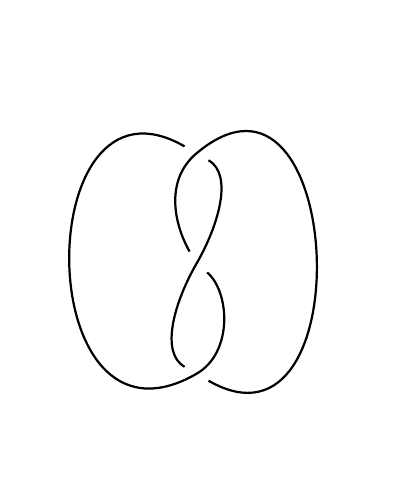
\begin{tikzpicture}[scale=0.7]
\coordinate (top) at (0,2);
\coordinate (mid) at (0,0);
\coordinate (bot) at (0,-2);
\draw [thick, shorten <= 5, shorten >= 5] (mid) to [out=120, in=-140] (top) to [out=40, in=-30, distance=100] (bot);
\draw [thick, shorten <=5, shorten >= 5] (bot) to [out=150, in=-120] (mid) to [out=60, in=-30] (top);
\draw [thick, shorten <=5, shorten >=5] (top) to [out=150, in =-150, distance=100] (bot) to [out=30, in=-40] (mid);
\end{tikzpicture}
\caption{}
\label{fig:trefoil}
\end{subfigure}\hfill% don't remove this comment or the subfigures stack!
\begin{subfigure}[b]{0.3\linewidth}
\captionsetup{skip=-20pt}
\centering
\begin{tikzpicture}[scale=0.7]
\coordinate (top) at (0,2);
\coordinate (mid) at (0,0);
\coordinate (bot) at (0,-2);
\draw [thick, shorten <= 5, shorten >= 5, -<-=0.13, -<-=0.52] (mid) to [out=120, in=-140] (top) to [out=40, in=-30, distance=100] (bot);
\draw [thick, shorten <=5, shorten >= 5, -<-=0.3, -<-=0.8] (bot) to [out=150, in=-120] (mid) to [out=60, in=-30] (top);
\draw [thick, shorten <=5, shorten >=5, -<-=0.3, -<-=0.9] (top) to [out=150, in =-150, distance=100] (bot) to [out=30, in=-40] (mid);
\end{tikzpicture}
\caption{}
\label{fig:oriented trefoil}
\end{subfigure}\hfill% same here!
\begin{subfigure}[b]{0.3\linewidth}
\captionsetup{skip=-20pt}
\centering
\begin{tikzpicture}[scale=0.7] %trefoil with eliminated crossings
\coordinate (topl) at (0,2);
\coordinate (midl) at (0,0);
\coordinate (botl) at (0,-2);
\coordinate (topr) at (0.25, 2);
\coordinate (midr) at (0.25,0);
\coordinate (botr) at (0.25,-2);
\draw [thick, -<-=0.45] (midl) to [out=120, in=-140] (topl) to [out=150, in =-150, distance=100] (botl) to [out=150, in=-120] (midl);
\draw [thick, -<-=0.45] (midr) to [out=60, in=-30] (topr) to [out=40, in=-30, distance=100] (botr) to [out=30, in=-40] (midr);
\end{tikzpicture}
\caption{}
\label{fig:crossing elimination}
\end{subfigure}
\caption{The trefoil knot, (a) without orientation, (b) with orientation, (c) with eliminated crossings.}
\label{fig:trefoil oriented crossing elimination}
\end{figure}
%%------------------------------------------------Seifert Figures 1------------------------------------------------------------------------------%%
\begin{figure}
\centering
\begin{subfigure}[b]{0.5\linewidth}
\captionsetup{skip=-50pt}
\centering
\begin{tikzpicture}[scale=0.75] %the trefoil as discs with twisted bands
%central coordinates
\coordinate (mid) at (0,0); \coordinate (top) at (0,1.5); \coordinate (bot) at (0,-1.5);
%left coordinates
\coordinate (topl1) at (-1,1.75); \coordinate (botl1) at (-1,1.25); \coordinate (topl2) at (-1,0.25); \coordinate (botl2) at (-1,-0.25); \coordinate (topl3) at (-1,-1.25); \coordinate (botl3) at (-1,-1.75);
%right coordinates
\coordinate (topr1) at (1,1.75); \coordinate (botr1) at (1,1.25); \coordinate (topr2) at (1,0.25); \coordinate (botr2) at (1,-0.25); \coordinate (topr3) at (1,-1.25); \coordinate (botr3) at (1,-1.75);
%top band
\draw [thick, ->-=0.3, ->-=0.8] (topr1) to [out=180, in=45] (top) to [out=-135, in=0] (botl1);
\draw [thick, shorten >=5,  -<-=0.5] (botr1) to [out=180, in =-45] (top);
\draw [thick, shorten <=5,  -<-=0.5] (top) to [out=135, in=0] (topl1);
%mid band
\draw [thick, ->-=0.3, ->-=0.8] (topr2) to [out=180, in=45] (mid) to [out=-135, in=0] (botl2);
\draw [thick, shorten >=5, -<-=0.5] (botr2) to [out=180, in =-45] (mid);
\draw [thick, shorten <=5,  -<-=0.5] (mid) to [out=135, in=0] (topl2);
%bot band
\draw [thick, ->-=0.3, ->-=0.8] (topr3) to [out=180, in=45] (bot) to [out=-135, in=0] (botl3);
\draw [thick, shorten >=5,  -<-=0.5] (botr3) to [out=180, in =-45] (bot);
\draw [thick, shorten <=5,  -<-=0.5] (bot) to [out=135, in=0] (topl3);
%left disc
\draw [thick] (topl3) to [out=85, in=-85] (botl2);
\draw [thick] (topl2) to [out=85, in=-85] (botl1);
\draw [thick, -<-=0.4] (topl1) to [out=125, in=-125, distance=100] (botl3);
%right disc
\draw [thick] (topr3) to [out=95, in=-95] (botr2);
\draw [thick] (topr2) to [out=95, in=-95] (botr1);
\draw [thick, -<-=0.4] (topr1) to [out=55, in=-55, distance=100] (botr3);
\end{tikzpicture}
\caption{}
\label{fig:seifert discs}
\end{subfigure}\hfill% stay!
\begin{subfigure}[b]{0.5\linewidth}
\captionsetup{skip=-50pt}
\centering
\begin{tikzpicture}[scale=0.75]
%central coordinates
\coordinate (top) at (0,1.5); \coordinate (bot) at (0,-1.5);
%left coordinates
\coordinate (topl1) at (-1,1.75); \coordinate (botl1) at (-1,1.25); \coordinate (topl3) at (-1,-1.25); \coordinate (botl3) at (-1,-1.75);
%right coordinates
\coordinate (topr1) at (1,1.75); \coordinate (botr1) at (1,1.25); \coordinate (topr2) at (1,0.25); \coordinate (botr2) at (1,-0.25); \coordinate (topr3) at (1,-1.25); \coordinate (botr3) at (1,-1.75);
%far right coordinates
\coordinate (twistfr) at (5,1.75); \coordinate (twistfr+) at (5.1,2.15);
\coordinate (topfr) at (4,0.5); \coordinate (botfr) at (4,-0.5);
%extra mid band coordinates
\coordinate (extopr) at (1,0.5); \coordinate (exbotr) at (1,0); \coordinate (extopl) at (2.35,1.4); \coordinate (exbotl) at (2.4, 1); \coordinate (extopm) at (2.4, -1); \coordinate (exbotm) at (2.35,-1.4);
\coordinate (exbotr-) at (0.95,-.15); \coordinate (topr2-) at (0.95,0.3);

%top band
\draw [thick, ->-=0.3, ->-=0.8] (topr1) to [out=180, in=45] (top) to [out=-135, in=0] (botl1);
\draw [thick, shorten >=5,  -<-=0.5] (botr1) to [out=180, in =-45] (top);
\draw [thick, shorten <=5,  -<-=0.5] (top) to [out=135, in=0] (topl1);
%bot band
\draw [thick, ->-=0.3, ->-=0.8] (topr3) to [out=180, in=45] (bot) to [out=-135, in=0] (botl3);
\draw [thick, shorten >=5,  -<-=0.5] (botr3) to [out=180, in =-45] (bot);
\draw [thick, shorten <=5,  -<-=0.5] (bot) to [out=135, in=0] (topl3);
%mid band
\draw [thick] (botr2) to [out=180, in=-125] (exbotr);
\draw [thick, -<-=0.6] (exbotr) to [out=55, in=-155] (exbotl);
\draw [thick, shorten >=3, -<-=0.2, -<-=0.7] (exbotl) to [out=25, in=-170] (twistfr) to [out=10, in=45, distance=25] (topfr) to [out=-125, in=125] (botfr);
\draw[thick, shorten <=3, -<-=0.5] (botfr) to [out=-45, in=0] (exbotm);
\draw [thick] (topr2-) to [out=92, in=-125] (extopr);
\draw [thick, ->-=0.5] (extopr) to [out=55, in=-155] (extopl);
\draw [thick, ->-=0.5] (extopl) to [out=25, in=-175] (twistfr+);
\draw [thick, shorten >=3, shorten <=3, ->-=0.5] (twistfr) to [out=-135, in=135] (topfr);
\draw [thick, shorten <=3, ->-=0.7] (topfr) to [out=-30, in=55] (botfr) to [out=-135, in=0] (extopm);
\draw [thin] (twistfr+) to [out=0, in=90] (5.3,1.73);
%left disc
\draw [thick] (topl3) to [out=85, in=-85] (botl1);
\draw [thick, -<-=0.4] (topl1) to [out=125, in=-125, distance=100] (botl3);
%right disc
\draw [thick] (topr3) to [out=95, in=-95] (botr2);
\draw [thin] (exbotr-) to [out=92, in=-92] (topr2-);
\draw [thick] (extopr) to [out=95, in=-95] (botr1);
\draw [thick, shorten >=2] (topr1) to [out=55, in=105, distance=25] (extopl);
\draw [thick, shorten <=2] (exbotl) to [out=-87, in=87] (extopm);
\draw [thick] (exbotm) to [out=-105, in=-55, distance=25] (botr3);
\end{tikzpicture}
\caption{}
\label{fig:seifert deform 1}
\end{subfigure}
\caption{(a) Seifert surface as discs connected with twisted bands. (b) Deforming the surface by sliding one end of the central band onto the same disc as its opposite end. Note the central band collects an extra half-twist as it slides around the edge of the top band.}
\end{figure}

%%------------------------------------------------Seifert Figures 2------------------------------------------------------------------------------%%

\begin{figure}
\centering
\begin{tikzpicture}
%central connection coords
\coordinate (topl) at (-0.25,0.25); \coordinate (topr) at (0.25, 0.25);, \coordinate (botl) at (-0.25, -0.25); \coordinate (botr) at (0.25,-0.25);

%horizontal band coords
\coordinate (htopl) at (-1.25,0.5); \coordinate (hbotl) at (-1.2,0.1); \coordinate (hmidl) at (-1.25, 0); \coordinate (hbotl-) at (-1.1,-0.14);
\coordinate (hmidtl) at (-0.25,1.3); \coordinate (hmidbl) at (-0.25, 0.8);
\coordinate (hmidtr) at (0.25, 1.5); \coordinate (hmidbr) at (0.25, 1);
\coordinate (hlefttop) at (3.05,3); \coordinate (hlefttopl) at (3.35, 2.7);
\coordinate (hrighttop) at (3.05,2.65); \coordinate (hrighttopm) at (2.9,1.6); \coordinate (hrighttopb) at (2.9,0.5);
\coordinate (hextra) at (3.4,2.6);
%vertical band coords
\coordinate (vtopl) at (-0.25,3); \coordinate (vtopr) at (0.25, 2.8); \coordinate (vtopm) at (-0.08,2.6);
\coordinate (vcrosst) at (-2.5, 1.5); \coordinate (vcrossb) at (-2.5,0);
\coordinate (vbotl) at (-0.25, -2.5); \coordinate (vbotr) at (0.25,-2.3); \coordinate (vbotm) at (-0.1, -2.1);
%horizontal band draw
\draw [thick, shorten >=9, ->-=0.5] (topl) to [out=180, in=-80] (htopl);
\draw [thick, distance=19, shorten <=7, ->-=0.7] (hmidl) to [out=95, in=-160] (hmidtl);
\draw [thick, ->-=0.5] (hmidtl) to [out=20,in=-160] (hmidtr) to [out=20, in=-170] (hlefttop);
\draw [thin] (hlefttop)  to [out=-10, in=90] (hextra);
\draw [thin, shorten <=-2] (hbotl-) to [out=150, in=-95] (htopl);

\draw [thick, -<-=0.2, -<-=0.8] (botl) to [out=180, in=-85] (hbotl) to [out=95, in=-160] (hmidbl);
\draw [thick, distance=10, -<-=0.5] (hmidbl) to [out=20, in=-160] (hmidbr) to [out=20, in=160] (hlefttopl);

\draw [thick, shorten >=2, ->-=0.5] (hrighttop) to [out =-100, in=135] (hrighttopm);
\draw [thick, shorten <=2, distance=15, ->-=0.2, ->-=0.65] (hrighttopm) to [out=-45, in=45] (hrighttopb) to [out=-135, in=0] (topr);
\draw [thick, shorten >=2, distance=10, -<-=0.3, -<-=0.8] (hlefttopl) to [out=-60, in=45] (hrighttopm) to [out=-135, in=135] (hrighttopb);
\draw [thick, shorten <=2, distance=30, -<-=0.55] (hrighttopb) to [out=-45, in=0] (botr);
%vertical band draw
\draw [thick, shorten >=2, -<-=0.5] (topl) to [out=90,in=-90] (hmidbl); \draw [thick, shorten >=2, ->-=0.5] (topr) to [out=90, in=-90] (hmidbr);
\draw [thick, shorten <=2, distance=12, -<-=0.5] (hmidtl) to [out=90, in=0] (vtopl);
\draw [thick, shorten <=2, distance=11, ->-=0.5] (hmidtr) to [out=90, in=-40] (vtopr);
\draw [thin] (vtopr) to [out=140, in=0] (vtopl);

\draw [thick, distance=13, shorten >=2, ->-=0.35, ->-=0.8] (vtopm) to [out=180, in=45] (vcrosst) to [out=-135,in=135] (vcrossb);
\draw [thick, shorten >=2, distance=22, -<-=0.5] (vtopl) to [out=180, in=135] (vcrosst);
\draw [thick, shorten <=2, -<-=0.5] (vcrosst) to [out=-45, in=45] (vcrossb);
\draw [thick, distance=25, -<-=0.5] (vcrossb) to [out=-135, in=180] (vbotl);
\draw [thick, shorten <=2, distance=25, ->-=0.5] (vcrossb) to [out=-45,in=180] (vbotm);
\draw [thick, distance=10, -<-=0.5] (vbotl) to [out=0, in=-90] (botl);
\draw [thick, distance=10, ->-=0.5] (vbotr) to [out=30, in=-90] (botr);
\draw [thin] (vbotl) to [out=0, in=-150] (vbotr);
%disc draw
\draw[thin, dashed] (0,0) circle (0.35); 
\end{tikzpicture}
%\begin{tikzpicture}
%%central connection coords
%\coordinate (topl) at (-0.25,0.25); \coordinate (topr) at (0.25, 0.25);, \coordinate (botl) at (-0.25, -0.25); \coordinate (botr) at (0.25,-0.25);
%%horizontal band coords
%\coordinate (htopl) at (-1.25,0.25); \coordinate (hbotl) at (-1.2,0.1); \coordinate (hmidl) at (-1.25, 0);
%\coordinate (hmidtl) at (-0.25,1.3); \coordinate (hmidbl) at (-0.25, 0.8);
%\coordinate (hmidtr) at (0.25, 1.5); \coordinate (hmidbr) at (0.25, 1);
%\coordinate (hlefttop) at (3.05,3); \coordinate (hlefttopl) at (3.35, 2.7);
%\coordinate (hrighttop) at (3.05,2.65); \coordinate (hrighttopm) at (2.9,1.6); \coordinate (hrighttopb) at (2.9,0.5);
%\coordinate (hextra) at (3.4,2.6);
%%vertical band coords
%\coordinate (vtopl) at (-0.25,3); \coordinate (vtopr) at (0.25, 2.5); \coordinate (vtopm) at (-0.08,2.6);
%\coordinate (vcrosst) at (-2.5, 1.5); \coordinate (vcrossb) at (-2.5,0);
%\coordinate (vbotl) at (-0.25, -2.5); \coordinate (vbotr) at (0.2,-2); \coordinate (vbotm) at (-0.1, -2.1);
%%horizontal band draw
%\draw [thick, shorten >=3, ->-=0.5] (topl) to [out=180, in=-10] (htopl);
%\draw [thick, shorten <=1, distance=20, ->-=0.7] (htopl) to [out=170, in=-160] (hmidtl);
%\draw [thick, ->-=0.5, shorten >=2] (hmidtl) to [out=20,in=-160] (hmidtr) to [out=20, in=-170] (hlefttop) to [out=10, in=45] (hrighttop);
%
%\draw [thick, -<-=0.2, -<-=0.8] (botl) to [out=180, in=-70] (hbotl) to [out=110, in=-160] (hmidbl);
%\draw [thick, distance=10, -<-=0.5] (hmidbl) to [out=20, in=-160] (hmidbr) to [out=20, in=160] (hlefttopl);
%
%\draw [thick, shorten <=2, shorten >=2, ->-=0.5] (hrighttop) to [out =-100, in=135] (hrighttopm);
%\draw [thick, shorten <=2, distance=15, ->-=0.2, ->-=0.65] (hrighttopm) to [out=-45, in=45] (hrighttopb) to [out=-135, in=0] (topr);
%\draw [thick, shorten >=2, distance=10, -<-=0.3, -<-=0.8] (hlefttopl) to [out=-60, in=45] (hrighttopm) to [out=-135, in=135] (hrighttopb);
%\draw [thick, shorten <=2, distance=30, -<-=0.55] (hrighttopb) to [out=-45, in=0] (botr);
%%vertical band draw
%\draw [thick, shorten >=2, -<-=0.5] (topl) to [out=90,in=-90] (hmidbl); \draw [thick, shorten >=2, ->-=0.5] (topr) to [out=90, in=-90] (hmidbr);
%\draw [thick, shorten <=2, distance=12, -<-=0.5] (hmidtl) to [out=90, in=0] (vtopl);
%\draw [thick, shorten <=2, shorten >=2, ->-=0.5] (hmidtr) to [out=90, in=-45] (vtopr) to [out=135, in=0] (vtopm);
%
%\draw [thick, distance=13, shorten <=2, shorten >=2, ->-=0.35, ->-=0.8] (vtopm) to [out=180, in=45] (vcrosst) to [out=-135,in=135] (vcrossb);
%\draw [thick, shorten >=2, distance=22, -<-=0.5] (vtopl) to [out=180, in=135] (vcrosst);
%\draw [thick, shorten <=2, -<-=0.5] (vcrosst) to [out=-45, in=45] (vcrossb);
%\draw [thick, distance=25, -<-=0.5] (vcrossb) to [out=-135, in=180] (vbotl);
%\draw [thick, shorten <=2, shorten >=2, distance=25, ->-=0.5] (vcrossb) to [out=-45,in=180] (vbotm);
%\draw [thick, distance=10, -<-=0.5] (vbotl) to [out=0, in=-90] (botl);
%\draw [thick, shorten <=2, ->-=0.5] (vbotm) to [out=0, in=-135] (vbotr) to [out=45, in=-90] (botr);
%
%
%\end{tikzpicture}
\caption{Shrinking both discs down results in two connected bands with two half-twists in each. The dashed circle represents the right disc in Fig (\ref{fig:seifert deform 1}).}
\label{fig:seifert deform 2}
\end{figure}

\begin{figure}
\centering
\begin{subfigure}[b]{0.5\linewidth}
	\centering
	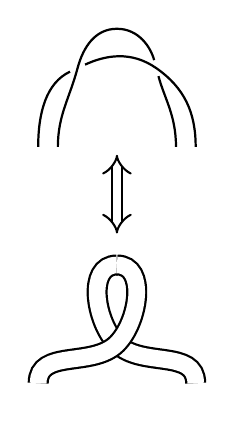
\begin{tikzpicture}
	%twisted band
	\draw[thick, shorten >=3] (0,0) to [out=90, in=-155] (0.5,1);
	\draw[thick, shorten >=3] (0.25,0) to [out=90, in=-105] (0.5,1) to [out=75, in=180] (1,1.5) to [out=0, in=105] (1.5,1);
	\draw[thick, shorten <=3] (0.5, 1) to [out=25, in=145] (1.5,1) to [out=-35, in=90] (2,0);
	\draw[thick, shorten <=3] (1.5,1) to [out=-75, in=90](1.75,0);
	%arrow
	\draw [line width =0.75pt, double distance=3pt, >=implies, <->] (1,-0.1) to (1,-1.1);
	%curl
	\draw[thick, double distance=6pt] (1,-1.5) to [out=180, in=135] (1,-2.5) to [out=-45, in=90] (2,-3);
	\draw[thick, double distance=6pt] (0,-3) to [out=90, in=-135] (1,-2.5) to [out=45,in=0] (1,-1.5);
	\end{tikzpicture}
	\caption{}
	\label{fig:twists to curl}
\end{subfigure}%
\begin{subfigure}[b]{0.5\linewidth}
	\centering
	\begin{tikzpicture}[scale=2, xscale=-1]
	%'disc' coordinates
	\coordinate (topl) at (-1,0); \coordinate (topr) at (1,0); \coordinate (botl) at (-1,-0.5); \coordinate (botr) at (1, -0.5);
	\coordinate (breakl1) at (-0.65,0); \coordinate (breakl2) at (-0.5,0); \coordinate (breakml1) at (-0.25,0); \coordinate (breakml2) at (-0.1,0); \coordinate (breakmr1) at (0.1,0); 	\coordinate (breakmr2) at (0.25,0); \coordinate (breakr1) at (0.5,0); \coordinate (breakr2) at (0.65,0);
	%draw `disc'
	\draw[thick, rounded corners] (breakl2) -- (breakml1);
	\draw[thick, rounded corners] (breakml2) -- (breakmr1);
	\draw[thick, rounded corners] (breakmr2) -- (breakr1); 
	\draw[thick, rounded corners, ->-=0.51] (breakr2) -- (topr) -- (botr) -- (botl) -- (topl) -- (breakl1);
	%band coords
	\coordinate (breakmidl) at (-0.575,0); \coordinate (breakmidmr) at (0.175,0); \coordinate (breakmidml) at (-0.175,0); \coordinate (breakmidr) at (0.575,0);
	\coordinate (leftmidb) at (-0.3,0.775);
	\coordinate (leftmidt) at (-0.3,1.575);
	\coordinate (rightmidb) at (0.3,0.775);
	\coordinate (rightmidt) at (0.3,1.575);
	%left band draw
	\draw[thick, double distance=7pt] (breakmidl) to [out=90, in=-135] (leftmidb) to [out=45, in=0] (leftmidt);
	\draw[thick, double distance=7pt, shorten <=-1] (leftmidt) to [out=180,in=135] (leftmidb) to [out=-45, in=90] (breakmidmr);
	%right band draw
	\draw[thick, double distance=7pt] (breakmidml) to [out=90, in=-135] (rightmidb) to [out=45, in=0] (rightmidt);
	\draw[thick,double distance=7pt, shorten <=-1] (rightmidt) to [out=180,in=135] (rightmidb) to [out=-45, in=90] (breakmidr);
	\end{tikzpicture}
	\caption{}
	\label{fig:trefoil curl}
\end{subfigure}
\caption{(a) We can deform two half-twists into a curl, and vice-versa. We use this technique on the trefoil in Fig (\ref{fig:seifert deform 2}) and deform further to get (b).}
\end{figure}

%%------------------------------------------------My Knot Talkthrough----------------------------------------------------------------------------%%
 Fig (\ref{fig:my knot}) is a knot diagram of the $5_2$ knot, and Fig (\ref{fig:my knot no crossings}) shows that the Seifert surface will have four oriented discs rather than the two we saw in the case of the trefoil. Fig (\ref{fig:my knot seifert deform 1}) presents the $5_2$ knot after the earlier process with the trefoil knot in Fig (\ref{fig:seifert deform 2}) has been completed; however, note the additional half-twists in the left/vertical band. We can transform this into a `tablet' in the same way as for the trefoil knot to get Fig (\ref{fig:my knot tablet 1}), but we could get rid of the double curl; ideally, we want only single curls or straight bands on the tablet, as  we then have a standard form.\\

This is where we can apply the notion of a pass-move to the bands. \textcolor{red}{Since a Seifert surface is oriented,} we can move one band through another band to perform a pass-move, as shown in Fig (\ref{fig:belt}). Whatever knot we are left with after completing the pass-move is pass-equivalent to the oriented knot we began with. Performing a pass-move on the knot in Fig (\ref{fig:my knot tablet 1}), we get the knot shown in Fig (\ref{fig:my knot tablet 2}); if we slide the neck of the far-right band to the left, travelling around the outside of the leftmost band, then rearrange, we get Fig (\ref{fig:my knot tablet 3}), which appears very different to the trefoil tablet. In fact, if we invert the procedure of turning a knot into a tablet, we will end up with the unknot. Fig (\ref{fig:passeq52}) shows this process.\\
%%------------------------------------------------My Knot Figures------------------------------------------------------------------------------%%
\begin{figure}
\centering
	\begin{subfigure}[b]{0.3\linewidth}
	\centering
	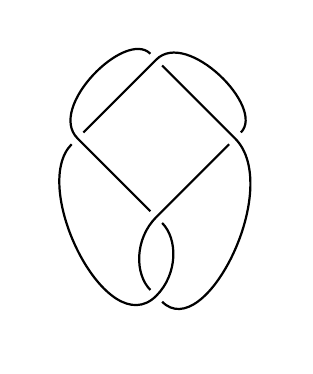
\begin{tikzpicture}
	\coordinate (top) at (0,2); \coordinate (topl) at (-1, 1); \coordinate (topr) at (1, 1); \coordinate (mid) at (0,0); \coordinate (bot) at (0,-1);
	\draw[thick, shorten <=3, shorten >=3] (bot) to [out=135,in=-135] (mid) to [out=45, in=-135] (topr);
	\draw[thick, shorten <=3, shorten >=3] (topr) to [out=45, in=45] (top) to [out=-135, in=45] (topl);
	\draw[thick, shorten <=3, shorten >=3] (topl) to [out=-135,in=-135] (bot) to [out=45, in=-45] (mid);
	\draw[thick, shorten <=3, shorten >=3] (mid) to [out=135,in=-45] (topl) to [out=135, in=135] (top);
	\draw[thick, shorten <=3, shorten >=3] (top) to [out=-45, in=135] (topr) to [out=-45, in=-45] (bot);
	\end{tikzpicture}
	\caption{}
	\label{fig:my knot}
	\end{subfigure}\hfill%
	\begin{subfigure}[b]{0.3\linewidth}
	\centering
	\begin{tikzpicture}
	\coordinate (top) at (0,2); \coordinate (topl) at (-1, 1); \coordinate (topr) at (1, 1); \coordinate (mid) at (0,0); \coordinate (bot) at (0,-1);
	\draw[thick,->-=0.2, ->-=0.75, shorten <=3, shorten >=3] (bot) to [out=135,in=-135] (mid) to [out=45, in=-135] (topr);
	\draw[thick, ->-=0.3, ->-=0.8, shorten <=3, shorten >=3] (topr) to [out=45, in=45] (top) to [out=-135, in=45] (topl);
	\draw[thick, ->-=0.4, ->-=0.85, shorten <=3, shorten >=3] (topl) to [out=-135,in=-135] (bot) to [out=45, in=-45] (mid);
	\draw[thick, ->-=0.3, ->-=0.7, shorten <=3, shorten >=3] (mid) to [out=135,in=-45] (topl) to [out=135, in=135] (top);
	\draw[thick, ->-=0.25, ->-=0.7, shorten <=3, shorten >=3] (top) to [out=-45, in=135] (topr) to [out=-45, in=-45] (bot);
	\end{tikzpicture}
	\caption{}
	\label{fig:my knot oriented}
	\end{subfigure}\hfill%
	\begin{subfigure}[b]{0.3\linewidth}
	\centering
	\begin{tikzpicture}
	\coordinate (top1) at (-0.1,2);\coordinate (top2) at (0.1,2); \coordinate (topl1) at (-1, 1.1); \coordinate (topl2) at (-1, 0.9); \coordinate (topr1) at (1, 1.1); \coordinate (topr2) at (1, 0.9); \coordinate (mid1) at (-0.1,0); \coordinate (mid2) at (0.1,0); \coordinate (bot1) at (-0.1,-1);\coordinate (bot2) at (0.1,-1);
	\draw[thick, ->-=0.25, ->-=0.7] (top2) to [out=-45, in=135] (topr1) to [out=45,in=45] (top2);
	\draw[thick,->-=0.25, ->-=0.7] (top1) to [out=-135,in=45] (topl1) to [out=135, in=135] (top1);
	\draw[thick, ->-=0.3, ->-=0.65, ->-=0.9] (topl2) to [out=-135,in=-135] (bot1) to [out=135, in=-135] (mid1) to [out=135, in=-45] (topl2);
	\draw[thick, ->-=0.3, ->-=0.65, ->-=0.9] (topr2) to [out=-45, in=-45] (bot2) to [out=45, in=-45] (mid2) to [out=45, in=-135] (topr2);
	\end{tikzpicture}
	\caption{}
	\label{fig:my knot no crossings}
	\end{subfigure}%
\caption{The $5_2$ knot, (a) without orientation, (b) with orientation, (c) with eliminated crossings.}
\label{fig:my knot figures}
\end{figure}


%%------------------------------------------------My Knot Figures 2------------------------------------------------------------------------------%%
\begin{figure}
\centering
\begin{subfigure}[b]{0.5\linewidth}
\captionsetup{skip=-20pt}
\centering
\begin{tikzpicture}[scale=1.25]
%disc1 coords
\coordinate (1rt) at (0,2); \coordinate (1rb) at (0,1.75); \coordinate (1bl) at (-1,1.5); \coordinate (1br) at (-0.75, 1.5);
%disc2 coords
\coordinate (2lt) at (0.5,2); \coordinate (2lb) at (0.5,1.75); \coordinate (2br) at (1.5,1.5); \coordinate (2bl) at (1.25, 1.5);
%disc3 coords
\coordinate (3tl) at (-1, 1); \coordinate (3tr) at (-0.75, 1); \coordinate (3mtt) at (0,0); \coordinate (3mtb) at (0,-0.25); \coordinate (3mbt) at (0,-1); \coordinate (3mbb) at (0,-1.25);
%disc4 coords
\coordinate (4tr) at (1.5,1); \coordinate (4tl) at (1.25, 1); \coordinate (4mtt) at (0.5, 0); \coordinate (4mtb) at (0.5, -0.25); \coordinate (4mbt) at (0.5, -1); \coordinate (4mbb) at (0.5,-1.25);
%band coords
\coordinate (1to3) at (-0.875,1.25); \coordinate (1to2) at (0.25,1.875); \coordinate (2to4) at (1.375,1.25); \coordinate (3to4t) at (0.25,-0.125); \coordinate (3to4b) at (0.25,-1.125);
%draw disc 1
\draw[thick, distance=20, -<-=0.5] (1rt) to [out=90, in=180] (1bl); \draw[thick, distance=5, -<-=0.5] (1br) to [out=0, in=-90] (1rb);
%draw disc 2
\draw[thick, distance=20, -<-=0.5] (2lt) to [out=90, in=0] (2br); \draw[thick, distance=5, -<-=0.5] (2bl) to [out=180, in=-90] (2lb);
%draw disc 3
\draw[thick, ->-=0.5] (3tl) to [out=180, in=-90] (3mbb); \draw[thick, ->-=0.5] (3mbt) to [out=90, in=-90] (3mtb); \draw[thick, ->-=0.5] (3mtt) to [out=90, in=0]  (3tr);
%draw disc 4
\draw[thick, ->-=0.5] (4tr) to [out=0, in=-90] (4mbb); \draw[thick, ->-=0.5] (4mbt) to [out=90, in=-90] (4mtb); \draw[thick,->-=0.5] (4mtt) to [out=90, in=180] (4tl);
%draw bands
\draw[thick, shorten >=3] (1rt) to [out=0, in=135] (1to2); \draw[thick, shorten <=3] (1to2) to [out=-45, in=180] (2lb);
\draw[thick] (1rb) to [out=0, in=-135] (1to2) to [out=45, in=180] (2lt);
\draw[thick, shorten >=3] (1br) to [out=-90, in=45] (1to3); \draw[thick, shorten <=3] (1to3) to [out=-135, in=90] (3tl);
\draw[thick] (1bl) to [out=-90, in=135] (1to3) to [out=-45, in=90] (3tr);
\draw[thick, shorten >=3] (2br) to [out=-90, in=45] (2to4); \draw[thick, shorten <=3] (2to4) to [out=-135, in=90] (4tl);
\draw[thick] (2bl) to [out=-90, in=135] (2to4) to [out=-45, in=90] (4tr);
\draw[thick, shorten >=3] (3mtt) to [out=0, in=135] (3to4t); \draw[thick, shorten <=3] (3to4t) to [out=-45, in=180] (4mtb);
\draw[thick] (3mtb) to [out=0, in=-135] (3to4t) to [out=45, in=180] (4mtt);
\draw[thick, shorten >=3] (3mbt) to [out=0, in=135] (3to4b); \draw[thick, shorten <=3] (3to4b) to [out=-45, in=180] (4mbb);
\draw[thick] (3mbb) to [out=0, in=-135] (3to4b) to [out=45, in=180] (4mbt);
\end{tikzpicture}
\caption{}
\label{fig:my knot seifert}
\end{subfigure}\hfill%
\begin{subfigure}[b]{0.5\linewidth}
\centering
\begin{tikzpicture}[scale=0.9]
%central connection coords
\coordinate (topl) at (-0.25,0.25); \coordinate (topr) at (0.25, 0.25);, \coordinate (botl) at (-0.25, -0.25); \coordinate (botr) at (0.25,-0.25);
%horizontal band coords
\coordinate (htopl) at (-1.25,0.25); \coordinate (hbotl) at (-1.25,0); \coordinate (hmidl) at (-1.25, 0);
\coordinate (hmidtl) at (-0.25,1.3); \coordinate (hmidbl) at (-0.25, 0.8);
\coordinate (hmidtr) at (0.25, 1.5); \coordinate (hmidbr) at (0.25, 1);
\coordinate (hlefttop) at (3.05,3); \coordinate (hlefttopl) at (3.35, 2.7);
\coordinate (hrighttop) at (3.05,2.65); \coordinate (hrighttopm) at (2.9,1.6); \coordinate (hrighttopb) at (2.9,0.5);
\coordinate (hextra) at (3.4,2.6);
%vertical band coords
\coordinate (vtopl) at (-0.25,3); \coordinate (vtopr) at (0.26, 2.55); \coordinate (vtopm) at (-0.08,2.6);
\coordinate (vcrosst) at (-2.5, 2); \coordinate (vcrossb) at (-2.5,0.75);
\coordinate (vbotl) at (-0.25, -2.75); \coordinate (vbotr) at (0.26,-2.2); \coordinate (vbotm) at (-0.1, -2.35);
%new vertical band coords
\coordinate (vcrosst2) at (-2.5, -0.5); \coordinate (vcrossb2) at (-2.5, -1.75);
%horizontal band draw
\draw [thick, shorten >=3, ->-=0.5] (topl) to [out=180, in=-10] (htopl);
\draw [thick, shorten <=1, distance=20, ->-=0.7] (htopl) to [out=170, in=-160] (hmidtl);
\draw [thick, shorten >=2, ->-=0.5] (hmidtl) to [out=20,in=-160] (hmidtr) to [out=20, in=-170] (hlefttop) to [out=10,in=60] (hrighttop);

\draw [thick, -<-=0.2, -<-=0.8] (botl) to [out=180, in=-85] (hbotl) to [out=95, in=-160] (hmidbl);
\draw [thick, distance=10, -<-=0.5] (hmidbl) to [out=20, in=-160] (hmidbr) to [out=20, in=160] (hlefttopl);

\draw [thick, shorten <=2, shorten >=2, ->-=0.5] (hrighttop) to [out =-100, in=135] (hrighttopm);
\draw [thick, shorten <=2, distance=15, ->-=0.2, ->-=0.65] (hrighttopm) to [out=-45, in=45] (hrighttopb) to [out=-135, in=0] (topr);
\draw [thick, shorten >=2, distance=10, -<-=0.3, -<-=0.8] (hlefttopl) to [out=-60, in=45] (hrighttopm) to [out=-135, in=135] (hrighttopb);
\draw [thick, shorten <=2, distance=30, -<-=0.55] (hrighttopb) to [out=-45, in=0] (botr);
%vertical band draw
\draw [thick, shorten >=2, -<-=0.5] (topl) to [out=90,in=-90] (hmidbl); \draw [thick, shorten >=2, ->-=0.5] (topr) to [out=90, in=-90] (hmidbr);
\draw [thick, shorten <=2, distance=12, -<-=0.5] (hmidtl) to [out=90, in=0] (vtopl);
\draw [thick, shorten <=2, shorten >=2, ->-=0.5] (hmidtr) to [out=90, in=-45] (vtopr) to [out=135, in=0] (vtopm);

\draw [thick, distance=13, shorten <=2, shorten >=2, ->-=0.35, ->-=0.8] (vtopm) to [out=180, in=45] (vcrosst) to [out=-135,in=135] (vcrossb);
\draw [thick, shorten >=2, distance=22, -<-=0.5] (vtopl) to [out=180, in=135] (vcrosst);
\draw [thick, shorten <=2, shorten >=2, -<-=0.3, -<-=0.8] (vcrosst) to [out=-45, in=45] (vcrossb)to [out=-135, in=135] (vcrosst2);
\draw[thick, shorten <=2, shorten >=2, ->-=0.3, ->-=0.75] (vcrossb) to [out=-45, in=45] (vcrosst2) to [out=-135, in=135] (vcrossb2);
\draw[thick, shorten <=2, -<-=0.15, -<-=0.7] (vcrosst2) to [out=-45, in=45] (vcrossb2) to [out=-135, in=180] (vbotl); 

\draw [thick, shorten <=2, shorten >=2, ->-=0.5] (vcrossb2) to [out=-45,in=180] (vbotm);
\draw [thick, distance=10, -<-=0.5] (vbotl) to [out=0, in=-90] (botl);
\draw [thick, shorten <=2, ->-=0.5] (vbotm) to [out=0, in=-110] (vbotr) to [out=70, in=-90] (botr);

%disc draw
\draw[thin, dashed] (0,0) circle (0.35); 
\end{tikzpicture}
\caption{}
\label{fig:my knot seifert deform 1}
\end{subfigure}
\caption{(a) A Seifert surface of the oriented $5_2$ knot. (b) Moving the central twisted band around in a similar manner to Fig (\ref{fig:seifert deform 1}), and shrinking the discs down. The dotted circle represents the right disc in Fig (\ref{fig:my knot seifert}).}
\label{fig:my knot seifert figs}
\end{figure}
%%------------------------------------------------Belt Picture------------------------------------------------------------------------------%%
\begin{figure}
\centering
\begin{tikzpicture}[scale=1.5]
%coordinates
	%band starts
	\coordinate(bl1) at (-0.25,0);\coordinate(bl2) at (0.25,0); \coordinate (br2) at (2.75,0); \coordinate (br1) at (3.25,0);
	%band twists
	\coordinate(bltwist) at (0,1); \coordinate(tltwist) at (1,1.5); \coordinate (trtwist) at (2,1.5); \coordinate(brtwist) at (3,1);
	%thin wires
	\coordinate (w1b) at (-0.25,0.45); \coordinate (w1t) at (-0.05, 1.25); \coordinate (w2l) at (0.75, 1.6); \coordinate (w2r) at (1.3,1.68); \coordinate(w3l) at (1.6, 1.7); \coordinate (w3r) at (2.24,1.61); \coordinate (w4t) at (3.04, 1.23); \coordinate (w4b) at (3.25, 0.45);
	%band bottom
	\coordinate(north) at (1.5,-0.85); \coordinate (south) at (1.5,-1.65); \coordinate (east) at (1.9, -1.25); \coordinate (west) at (1.1,-1.25); \coordinate (west-) at (0.5,-1.85); \coordinate (south-) at (1, -2.15); \coordinate (east+) at (2.5, -1.85); \coordinate (south+) at (2,-2.15);
%drawing
	%band
	\draw[thick, shorten >=2, ->-=0.4, ->-=0.8] (bl1) to [out=90, in=-135] (bltwist) to [out=45, in=-135] (tltwist); \draw[thick, shorten <=2, shorten >=2, ->-=0.3, ->-=0.8] (tltwist) to [out=45, in=135] (trtwist) to [out=-45, in=135] (brtwist); \draw[thick, shorten <=2, ->-=0.7] (brtwist) to [out=-45, in=90] (br1);
	\draw[thick, shorten >=2, -<-=0.6] (bl2) to [out=90, in=-45] (bltwist); \draw[thick, shorten <=2, shorten >=2, -<-=0.3, -<-=0.8] (bltwist) to [out=135, in=135] (tltwist) to [out=-45, in=-135] (trtwist); \draw[thick, shorten <=2, -<-=0.3, -<-=0.8] (trtwist) to [out=45, in=45] (brtwist) to [out=-135, in=90] (br2);
	%dashing?
	\draw[line width=2, white,densely dotted, shorten <=0.5, shorten >=-2] (bltwist) to [out=135, in=-115] (w1t); \draw[line width=2, white,densely dotted, shorten <=0.5] (tltwist) to [out=45, in=-170] (w2r); \draw[line width=2, white,densely dotted, shorten <=0.5] (trtwist) to [out=45, in=180] (w3r); \draw[line width=2, white,densely dotted, shorten <=0.5] (brtwist) to [out=-45, in=95] (w4b);
	%wires
	\draw[thin, shorten >=-2] (w1b) to [out=90, in=-135] (w1t); \draw[thin] (w2l) to [out=0, in=180] (w2r);  \draw[thin] (w3l) to [out=0, in=180] (w3r);  \draw[thin] (w4t) to [out=-45, in=90] (w4b);
	%bottom crossing
	\draw[thick, -<-=0.3, -<-=0.7, -<-=0.9] (bl1) to [out=-90,in=135] (west) to [out=-45, in=135] (south) to [out=-45, in=135] (south+); \draw[thick, ->-=0.3, ->-=0.65, ->-=0.9] (bl2) to [out=-90,in=135] (north) to [out=-45, in=135] (east) to [out=-45, in=135] (east+);
	\draw[thick, shorten >=2, -<-=0.6] (br2) to [out=-90, in=45] (north); \draw[thick, densely dotted, shorten <=2, shorten >=2, -<-=0.55] (north) to [out=-135, in=45] (west); \draw[thick, shorten <=2, -<-=0.6] (west) to [out=-135, in=45] (west-);
	\draw[thick, shorten >=2, ->-=0.6] (br1) to [out=-90, in=45] (east); \draw[thick, densely dotted, shorten <=2, shorten >=2, ->-=0.6] (east) to [out=-135, in=45] (south); \draw[thick, shorten <=2, ->-=0.6] (south) to [out=-135, in=45] (south-);
\end{tikzpicture}
\caption{Passing the bands through each other at the lower crossing point negates the four half-twists. Note that each band edge is oppositely-oriented.}
\label{fig:belt}
\end{figure}


%%------------------------------------------------My Knot Tablet Form----------------------------------------------------------------------------%%
\begin{figure}
\centering
\begin{subfigure}{0.45\linewidth}
\centering
\begin{tikzpicture}[scale=2]
%'disc' coordinates
	\coordinate (topl) at (-1,0); \coordinate (topr) at (2,0); \coordinate (botl) at (-1,-0.5); \coordinate (botr) at (2, -0.5);
	\coordinate (breakl1) at (-0.65,0); \coordinate (breakl2) at (-0.5,0); \coordinate (breakml1) at (-0.25,0); \coordinate (breakml2) at (-0.1,0); \coordinate (breakmr1) at (0.1,0); 	\coordinate (breakmr2) at (0.25,0); \coordinate (breakr1) at (1.5,0); \coordinate (breakr2) at (1.65,0);
	%draw `disc'
	\draw[thick, rounded corners] (breakl2) -- (breakml1);
	\draw[thick, rounded corners] (breakml2) -- (breakmr1);
	\draw[thick, rounded corners] (breakmr2) -- (breakr1); 
	\draw[thick, rounded corners, -<-=0.5] (breakr2) -- (topr) -- (botr) -- (botl) -- (topl) -- (breakl1);
%band coords
	\coordinate (breakmidl1) at (-0.575,0); \coordinate (breakmidl2) at (-0.175,0); \coordinate (breakmidr2) at (0.175,0); \coordinate (breakmidr1) at (1.575,0);
	\coordinate (leftmidb) at (-0.3,0.775); \coordinate (leftmidt) at (-0.3,1.575);
	\coordinate (midmidb) at (0.3,0.775); \coordinate (midmidt) at (0.3,1.575); \coordinate (turn) at (0.75,0.5);
	\coordinate (rightmidb) at (1.25,0.775); \coordinate (rightmidt) at (1.25,1.575);
%left band draw
	\draw[thick, double distance=7pt] (breakmidl1) to [out=90, in=-135] (leftmidb) to [out=45, in=0] (leftmidt);
	\draw[thick, double distance=7pt, shorten <=-1] (leftmidt) to [out=180,in=135] (leftmidb) to [out=-45, in=90] (breakmidr2);
%right band draw
\draw[thick, double distance=7pt] (breakmidl2) to [out=90, in=-135] (midmidb) to [out=45, in=0] (midmidt);
\draw[thick, double distance=7pt, shorten <=-1] (midmidt) to [out=180, in=135] (midmidb) to [out=-45, in=180] (turn) to [out=0, in=-135] (rightmidb) to [out=45, in=0] (rightmidt);
\draw[thick, double distance=7pt, shorten <=-1] (rightmidt) to [out=180, in=135] (rightmidb) to [out=-45, in=90] (breakmidr1);	
\end{tikzpicture}
\caption{}
\label{fig:my knot tablet 1}
\end{subfigure}\hfill%
\begin{subfigure}{0.45\linewidth}
\centering
\begin{tikzpicture}[scale=2]
%'disc' coordinates
	\coordinate (topl) at (-1,0); \coordinate (topr) at (2,0); \coordinate (botl) at (-1,-0.5); \coordinate (botr) at (2, -0.5);
	\coordinate (breakl1) at (-0.65,0); \coordinate (breakl2) at (-0.5,0); \coordinate (breakml1) at (-0.25,0); \coordinate (breakml2) at (-0.1,0); \coordinate (breakmr1) at (0.1,0); 	\coordinate (breakmr2) at (0.25,0); \coordinate (breakr1) at (1.5,0); \coordinate (breakr2) at (1.65,0);
	%draw `disc'
	\draw[thick, rounded corners] (breakl2) -- (breakml1);
	\draw[thick, rounded corners] (breakml2) -- (breakmr1);
	\draw[thick, rounded corners] (breakmr2) -- (breakr1); 
	\draw[thick, rounded corners, -<-=0.5] (breakr2) -- (topr) -- (botr) -- (botl) -- (topl) -- (breakl1);
%band coords
	\coordinate (breakmidl1) at (-0.575,0); \coordinate (breakmidl2) at (-0.175,0); \coordinate (breakmidr2) at (0.175,0); \coordinate (breakmidr1) at (1.575,0);
	\coordinate (leftmidb) at (-0.3,0.775); \coordinate (leftmidt) at (-0.3,1.575);
	\coordinate (midmidb) at (0.3,0.775); \coordinate (midmidt) at (0.3,1.575); \coordinate (turn) at (0.75,0.5);
	\coordinate (rightmidb) at (1.25,0.775); \coordinate (rightmidt) at (1.25,1.575);
%left band draw
	\draw[thick, double distance=7pt] (breakmidl1) to [out=90, in=-135] (leftmidb) to [out=45, in=0] (leftmidt);
	\draw[thick, double distance=7pt, shorten <=-1] (leftmidt) to [out=180,in=135] (leftmidb) to [out=-45, in=90] (breakmidr2);
%right band draw
\draw[thick, double distance=7pt] (breakmidl2) to [out=90, in=-135] (midmidb) to [out=45, in=0] (midmidt);
\draw[thick, double distance=7pt] (rightmidt) to [out=180, in=135] (rightmidb) to [out=-45, in=90] (breakmidr1);	
\draw[thick, double distance=7pt, shorten <=-1, shorten >=-1] (midmidt) to [out=180, in=135] (midmidb) to [out=-45, in=180] (turn) to [out=0, in=-135] (rightmidb) to [out=45, in=0] (rightmidt);
\end{tikzpicture}
\caption{}
\label{fig:my knot tablet 2}
\end{subfigure}
\begin{subfigure}{0.5\linewidth}
\centering
\begin{tikzpicture}[scale=2]
%'disc' coordinates
\coordinate (topl) at (-1,0); \coordinate (topr) at (1,0); \coordinate (botl) at (-1,-0.5); \coordinate (botr) at (1, -0.5);
	\coordinate (breakl1) at (-0.65,0); \coordinate (breakl2) at (-0.5,0); \coordinate (breakml1) at (-0.25,0); \coordinate (breakml2) at (-0.1,0); \coordinate (breakmr1) at (0.1,0); 	\coordinate (breakmr2) at (0.25,0); \coordinate (breakr1) at (0.5,0); \coordinate (breakr2) at (0.65,0);
	%draw `disc'
	\draw[thick, rounded corners] (breakl2) -- (breakml1);
	\draw[thick, rounded corners] (breakml2) -- (breakmr1);
	\draw[thick, rounded corners] (breakmr2) -- (breakr1); 
	\draw[thick, rounded corners, -<-=0.5] (breakr2) -- (topr) -- (botr) -- (botl) -- (topl) -- (breakl1);
%band coords
	\coordinate (breakmidl) at (-0.575,0); \coordinate (breakmidmr) at (0.175,0); \coordinate (breakmidml) at (-0.175,0); \coordinate (breakmidr) at (0.575,0);
	\coordinate (leftmidb) at (-0.3,0.775);
	\coordinate (leftmidt) at (-0.3,1.575);
	\coordinate (rightmidb) at (0.3,0.775);
	\coordinate (rightmidt) at (0.3,1.575);
%left band draw
	\draw[thick, double distance=7pt] (breakmidl) to [out=90, in=-135] (leftmidb) to [out=45, in=0] (leftmidt);
	\draw[thick, double distance=7pt, shorten <=-1] (leftmidt) to [out=180,in=135] (leftmidb) to [out=-45, in=90] (breakmidmr);
%right band draw
	\draw[thick, double distance=7pt] (breakmidml) to [out=90, in=180] (rightmidb) to [out=0, in=90] (breakmidr);
\end{tikzpicture}
\caption{}
\label{fig:my knot tablet 3}
\end{subfigure}
\caption{a) The $5_2$ knot in tablet form. b) The result of a pass-move on the far-right crossing. c) A tablet for a knot that is pass-equivalent to the $5_2$ knot.}
\label{}
\end{figure}

%%------------------------------------------------Undoing My Knot----------------------------------------------------------------------------%%
 \begin{figure}
 \centering
 \begin{subfigure}{0.5\linewidth}
 \centering
 \begin{tikzpicture}[scale=2]
 %crossing coordinates
 	%top left doublet
 	\coordinate (lefttopt) at (-0.3,1.675); \coordinate (lefttopb) at (-0.3,1.5);
 	%left quartet
 	\coordinate (north) at (-0.3,1); \coordinate (south) at (-0.3,0.75); \coordinate (east) at (-0.175,0.875); \coordinate (west) at (-0.425,0.875);
 	%right quartet
 	\coordinate(rnorth) at (0,0.75); \coordinate(rsouth) at (0,0.5); \coordinate (reast) at (0.125,0.625); \coordinate (rwest) at (-0.125,0.625);
 	%right doublet
 	\coordinate (rightt) at (0.3,0.925); \coordinate (rightb) at (0.3,0.75);
%'disc' coordinates
	\coordinate (breakl1) at (-0.65,0); \coordinate (breakl2) at (-0.5,0); \coordinate (breakml1) at (-0.25,0); \coordinate (breakml2) at (-0.1,0); \coordinate (breakmr1) at (0.1,0); 	\coordinate (breakmr2) at (0.25,0); \coordinate (breakr1) at (0.5,0); \coordinate (breakr2) at (0.65,0);
%drawing
\draw[thick, shorten >=2] (breakl1) to [out=90, in=-135] (west);
\draw[thick, shorten >=2, shorten <=2] (west) to [out=45, in=-135] (north);
\draw[thick, shorten >=2, shorten <=2] (north) to [out=45,in=0] (lefttopb) to [out=180, in=135] (north) to [out=-45, in=135] (east) to [out=-45, in=135] (rnorth);
\draw[thick, shorten >=2, shorten <=2] (rnorth) to [out=-45, in=135] (reast);
\draw[thick, shorten >=2, shorten <=2] (reast) to [out=-45, in=90] (breakmr2) to [out=0, in=180] (breakr1) to [out=90, in=0] (rightb) to [out=180, in=45] (reast) to [out=-135, in=45] (rsouth) to [out=-135, in=90] (breakml2) to [out=0, in=180] (breakmr1) to [out=90, in=-45] (rsouth);
\draw[thick, shorten >=2, shorten <=2] (rsouth) to [out=135, in=-45] (rwest);
\draw[thick, shorten >=2, shorten <=2] (rwest) to [out=135, in=-45] (south) to [out=135, in=-45] (west) to [out=135, in=180] (lefttopt) to [out=0, in=45] (east);
\draw[thick, shorten >=2, shorten <=2] (east) to [out=-135, in=45] (south);
\draw[thick, shorten <=2, -<-=0.83] (south) to [out=-135, in=90] (breakl2) to [out=0, in=180] (breakml1) to [out=90, in=-135] (rwest) to [out=45, in=-135] (rnorth) to [out=45, in=180] (rightt) to [out=0, in=90] (breakr2) to [out=-90, in=-90] (breakl1);
 \end{tikzpicture}
 \label{fig:pass eq 52 1}
 \caption{}
 \end{subfigure}\hfill%
 \begin{subfigure}{0.5\linewidth}
 \centering
 \begin{tikzpicture}[scale=2]
  %crossing coordinates
 	%top left doublet
 	\coordinate (lefttopt) at (-0.3,1.675); \coordinate (lefttopb) at (-0.3,1.5);
 	%left quartet
 	\coordinate (northl) at (-0.35,1); \coordinate (northr) at (-0.25,1); \coordinate (south) at (-0.3,0.75); \coordinate (east) at (-0.175,0.875); \coordinate (west) at (-0.425,0.875);
 	%right quartet
 	\coordinate(rnorth) at (0,0.75); \coordinate(rsouthl) at (-0.1,0.5); \coordinate(rsouthr) at (0.1,0.5); \coordinate (reastt) at (0.125,0.675); \coordinate (reastb) at (0.125,0.575); \coordinate (rwest) at (-0.125,0.625);
 	%right doublet
 	\coordinate (rightt) at (0.3,0.925); \coordinate (rightb) at (0.3,0.75);
 	%extras
 	\coordinate (leftloop) at (0.4,0.3);
%'disc' coordinates
	\coordinate (breakl1) at (-0.65,0); \coordinate (breakl2) at (-0.5,0); \coordinate (breakml1) at (-0.25,0); \coordinate (breakml2) at (-0.1,0); \coordinate (breakmr1) at (0.1,0); 			\coordinate (breakmr2) at (0.25,0); \coordinate (breakr1) at (0.5,0); \coordinate (breakr2) at (0.65,0);
%drawing
\draw[thick, shorten >=2] (breakl1) to [out=90, in=-135] (west);
\draw[thick, shorten >=2, shorten <=2] (west) to [out=45, in=-135] (northl) to [out=90, in=180] (lefttopb) to [out=0, in=90] (northr) to [out=-45, in=135] (rnorth);
\draw[thick, shorten >=2, shorten <=2] (rnorth) to [out=-45, in=180] (reastt) to [out=0, in=180] (rightb) to[out=0, in=0] (leftloop) to [out=180, in=0] (reastb) to [out=-135, in=45] (rsouthr) to [out=180, in=0] (breakmr1) to [out=180, in=-90] (rsouthl) to [out=135, in=-45] (rwest);
\draw[thick, shorten >=4, shorten <=2] (rwest) to [out=135, in=-45] (south) to [out=135, in=-45] (west) to [out=135, in=180] (lefttopt) to [out=0, in=45] (east);
\draw[thick, shorten >=2] (east) to [out=-135, in=45] (south);
\draw[thick, shorten <=2, -<-=0.83] (south) to [out=-135, in=90] (breakl2) to [out=0, in=180] (breakml1) to [out=90, in=-135] (rwest) to [out=45, in=-135] (rnorth) to [out=45, in=180] (rightt) to [out=0, in=90] (breakr2) to [out=-90, in=-90] (breakl1);
 \end{tikzpicture}
 \label{fig:pass eq 52 2}
 \caption{}
 \end{subfigure}
 \begin{subfigure}{0.3\linewidth}
 \centering
 \begin{tikzpicture}[scale=2]
 %coordinates
 	%top left doublet
 	\coordinate (lefttopt) at (-0.3,1.675); \coordinate (lefttopb) at (-0.3,1.5);
 	%left quartet
 	\coordinate (northl) at (-0.35,1); \coordinate (northr) at (-0.25,1); \coordinate (south) at (-0.3,0.75); \coordinate (east) at (-0.175,0.875); \coordinate (west) at (-0.425,0.875);
 	%right doublet
 	\coordinate (rightt) at (0.3,0.925); \coordinate (rightb) at (0.2,0.5);
 	%bottom left
 	\coordinate (breakl1) at (-0.65,0); \coordinate (breakl2) at (-0.5,0);
 	%middle right
 	\coordinate(rnorth) at (0,0.75); \coordinate (rwest) at (-0.125,0.625);
%drawing
\draw[thick, shorten >=2] (breakl1) to [out=90, in=-135] (west);
\draw[thick, shorten >=4, shorten <=2] (west) to [out=45, in=-135] (northl) to [out=90, in=180] (lefttopb) to [out=0, in=90] (northr) to [out=-45, in=135] (rnorth) to [out=-45, in=45] (rightb) to [out=-135, in=-45] (rwest) to [out=135, in=-45] (south) to [out=135, in=-45] (west) to [out=135, in=180] (lefttopt) to [out=0, in=45] (east);
\draw[thick, shorten >=2] (east) to [out=-135, in=45] (south);
\draw[thick, shorten <=2, -<-=0.93] (south) to [out=-135, in=90] (breakl2) to [out=-90, in=-90] (breakl1);
 \end{tikzpicture}
 \label{fig:pass eq 52 3}
 \caption{}
 \end{subfigure}\hfill%
 \begin{subfigure}{0.3\linewidth}
 \centering
 \begin{tikzpicture}[scale=2]
 %coordinates
 	%top left doublet
 	\coordinate (lefttopt) at (-0.3,1.675); \coordinate (lefttopb) at (-0.3,1.5);
 	%left quartet
 	\coordinate (northl) at (-0.35,1); \coordinate (northr) at (-0.25,1); \coordinate (west) at (-0.425,0.875);
 	%bottom
 	\coordinate (breakl1) at (-0.65,0.4); \coordinate (far right) at (0.5,0.2);
 	%middle right
 	\coordinate(rnorth) at (0,0.75); \coordinate (rwest) at (-0.125,0.625);
%drawing
\draw[thick, shorten >=2] (breakl1) to [out=90, in=-135] (west);
\draw[thick, shorten <=2, -<-=0.88] (west) to [out=45, in=-135] (northl) to [out=90, in=180] (lefttopb) to [out=0, in=90] (northr) to [out=-45, in=135] (rnorth) to [out=-45, in=45] (rightb) to [out=-135, in=-45] (rwest) to [out=135, in=-45] (south) to [out=135, in=-45] (west) to [out=135, in=180] (lefttopt) to [out=0, in=45] (far right) to [out=-135, in=-90] (breakl1);
 \end{tikzpicture}
 \label{fig:pass-eq 52 4}
 \caption{}
 \end{subfigure}\hfill%
  \begin{subfigure}{0.3\linewidth}
 \centering
 \begin{tikzpicture}[scale=2]
 %coordinates
 	\coordinate (tl) at (-0.3, 1.675); \coordinate (mr) at (0.5, 0.2); \coordinate (bl) at (-0.65,0.4); \coordinate (mb) at (-0.1, 0.75); \coordinate (mt) at (-0.1, 0.85);
%drawing
\draw[thick, -<-=0.51] (tl) to [out=0, in=45] (mr) to [out=-135, in=-90] (bl) to [out=90, in=-135] (mb) to [out=45, in=-45] (mt) to [out=135, in=180] (tl);
  \end{tikzpicture}
 \label{fig:pass eq 52 5}
 \caption{}
 \end{subfigure}
 \caption{(a) Fig (\ref{fig:my knot tablet 3}) as a knot. (b) Type 1 Reidemeister moves used to untwist the three inner loops. (c) Type 2 Reidemeister move used to slide the large right loop over the small right loop. (d) Type 2 Reidemeister move used to slide the rightmost below strand out from under the small right loop. (e) Type 1 Reidemeister move used to untwist the remaining loop.}
\label{fig:passeq52}
\end{figure}

%%------------------------------------------------Trefoil Composition----------------------------------------------------------------------------%%
So far we have shown that a tablet with two curls is is bounded by the trefoil knot, and a tablet with one curl and one straight band is bounded by the unknot. We know the composition of the two will also be bounded by the trefoil, as any knot composed with the unknot just returns the original knot. [THEOREM?] This means we have two cases left to examine; a tablet with two straight bands, and a tablet with two or more sets of two curls (i.e. a composition of trefoils).\\
\\
The first case is the simpler, as we can convert such a tablet back into a knot diagram; Fig (\ref{fig:2-band tablet to unknot}) shows this process. This means that any composition of this tablet with another will just return the original tablet, so we can move on.\\
\\
The second case requires establishing that the trefoil is pass-equivalent to its mirror image. If we return to the tablet form of the trefoil in Fig (\ref{fig:trefoil curl}), we can perform a pass-move at each set of band crossings, then convert back to a knot diagram and rearrange to a configuration more like Fig (\ref{fig:oriented trefoil}); Fig (\ref{fig:pass move mirror trefoil tablet to knot}) shows this process. We note that the two trefoils are mirrors of each other; reversing the orientation of one trefoil gives us the second. The trefoil is therefore \emph{chiral} [DEFINITION?]). We have thus demonstrated the trefoil is pass equivalent to its mirror image.\\
\\
The result of this demonstration is that two trefoils composed together are pass equivalent to a trefoil composed with its mirror image. If we can show that this knot composition is pass-equivalent to either the unknot or to the trefoil knot (mirror or otherwise), then we have a result for every tablet case, and the Arf invariant is therefore well-defined.\\
\\
\textcolor{red}{pic of trefoil composition pass equivalence to unknot here}

%%------------------------------------------------Tablet to Unknot Pic----------------------------------------------------------------------------%%
\begin{figure}
\centering
\begin{subfigure}[b]{0.5\linewidth}
	\centering
	\begin{tikzpicture}[scale=2]
	%'disc' coordinates
	\coordinate (topl) at (-1,0); \coordinate (topr) at (1,0); \coordinate (botl) at (-1,-0.5); \coordinate (botr) at (1, -0.5);
	\coordinate (breakl1) at (-0.65,0); \coordinate (breakl2) at (-0.5,0); \coordinate (breakml1) at (-0.25,0); \coordinate (breakml2) at (-0.1,0); \coordinate (breakmr1) at (0.1,0); 	\coordinate (breakmr2) at (0.25,0); \coordinate (breakr1) at (0.5,0); \coordinate (breakr2) at (0.65,0);
	%draw `disc'
	\draw[thick, rounded corners] (breakl2) -- (breakml1);
	\draw[thick, rounded corners] (breakml2) -- (breakmr1);
	\draw[thick, rounded corners] (breakmr2) -- (breakr1); 
	\draw[thick, rounded corners, -<-=0.51] (breakr2) -- (topr) -- (botr) -- (botl) -- (topl) -- (breakl1);
	% band coordinates
	\coordinate (midbreakl1) at (-0.575,0); \coordinate (midbreakl2) at (-0.175,0); \coordinate (midbreakr1) at (0.175,0); \coordinate (midbreakr2) at (0.575,0);
	\coordinate (rightmidb) at (0.3,0.775); \coordinate (leftmidb) at (-0.3,0.775);
	%draw band
	\draw[thick, double distance=7pt] (midbreakl1) to [out=90, in=180] (leftmidb) to [out=0,in=90] (midbreakr1);
	\draw[thick, double distance=7pt] (midbreakl2) to [out=90, in=180] (rightmidb) to [out=0,in=90] (midbreakr2);
	\end{tikzpicture}
	\caption{}
	\label{fig:oriented tablet unknot}
\end{subfigure}

\begin{subfigure}[b]{0.33\linewidth}
	\centering
	\begin{tikzpicture}[scale=2]
	%'disc' coordinates
	\coordinate (breakl1) at (-0.65,0); \coordinate (breakl2) at (-0.5,0); \coordinate (breakml1) at (-0.25,0); \coordinate (breakml2) at (-0.1,0); \coordinate (breakmr1) at (0.1,0); \coordinate (breakmr2) at (0.25,0); \coordinate (breakr1) at (0.5,0); \coordinate (breakr2) at (0.65,0);
	%quartet
 	\coordinate(north) at (0,0.75); \coordinate(south) at (0,0.5); \coordinate (east) at (0.125,0.625); \coordinate (west) at (-0.125,0.625);
 	%right doublet
 	\coordinate (rightt) at (0.3,0.925); \coordinate (rightb) at (0.3,0.75);
 	%left doublet
 	\coordinate (leftt) at (-0.3,0.925); \coordinate (leftb) at (-0.3,0.75);
	%drawing
	\draw[thick, , -<-=0.51] (breakr2) to [out=-90, in=-90] (breakl1);
	\draw[thick, shorten >=2] (breakl1) to [out=90, in=180] (leftt) to [out=0, in=135] (north);
	\draw[thick, shorten >=2, shorten <=2] (north) to [out=-45, in=135] (east);
	\draw[thick, shorten <=2, shorten >=2] (east) to [out=-45, in=90] (breakmr2) to [out=0, in=-180] (breakr1) to [out=90, in=0] (rightb) to [out=180, in=45] (east) to [out=-135, in=45] (south) to [out=-135,  in=90] (breakml2) to [out=0, in=180] (breakmr1) to [out=90, in=-45] (south);
	\draw[thick, shorten >=2, shorten <=2] (south) to [out=135, in=-45] (west);
	\draw[thick, shorten <=2] (west) to [out=135, in=0] (leftb) to [out=180, in=90] (breakl2) to [out=0, in=180] (breakml1) to [out=90, in=-135] (west) to [out=45, in=-135] (north) to [out=45, in=180] (rightt) to [out=0, in=90] (breakr2);
	\end{tikzpicture}
	\caption{}
	\label{fig:oriented knot unknot 1}
\end{subfigure}%
\begin{subfigure}[b]{0.33\linewidth}
	\centering
	\begin{tikzpicture}[scale=2]
	%'disc' coordinates
	\coordinate (breakl1) at (-0.65,0); \coordinate (breakl2) at (-0.5,0); \coordinate (breakml1) at (-0.25,0); \coordinate (breakml2) at (-0.1,0); \coordinate (breakmr1) at (0.1,0); \coordinate (breakmr2) at (0.25,0); \coordinate (breakr1) at (0.5,0); \coordinate (breakr2) at (0.65,0);
	%quartet
 	\coordinate(north) at (0,0.75); \coordinate(southl) at (-0.05,0.5); \coordinate(southr) at (0.05,0.5); \coordinate (eastt) at (0.125,0.675); \coordinate (eastb) at (0.125,0.575); \coordinate (westt) at (-0.125,0.675); \coordinate (westb) at (-0.125,0.575);
 	%right doublet
 	\coordinate (rightt) at (0.3,0.925); \coordinate (rightb) at (0.3,0.75);
 	%left doublet
 	\coordinate (leftt) at (-0.3,0.925); \coordinate (leftb) at (-0.3,0.75);
 	%drawing
 	\draw[thick, -<-=0.51] (breakr2) to [out=-90, in=-90] (breakl1); \draw[thick, shorten >=2] (breakl1) to [out=90, in=180] (leftt) to [out=0, in=135] (north); \draw[thick, shorten <=2] (north) to [out=-45, in=135] (eastt) to [out=45, in=180] (rightb) to [out=0, in=90] (breakr1) to [out=180, in=0] (breakmr2) to [out=90, in=-45] (eastb) to [out=-135, in=45] (southr) to [out=-45, in=90] (breakmr1) to [out=180, in=0] (breakml2) to [out=90, in=-135] (southl) to [out=135, in=-45] (westb) to [out=-135, in=90] (breakml1) to [out=180, in=0] (breakl2) to [out=90, in=180] (leftb) to [out=0, in=135] (westt) to [out=45, in=-135] (north) to [out=45, in=180] (rightt) to [out=0, in=90] (breakr2);
	\end{tikzpicture}
	\caption{}
	\label{fig:oriented knot unknot 2}
\end{subfigure}%
\begin{subfigure}[b]{0.33\linewidth}
	\centering
	\begin{tikzpicture}[scale=2]
	%'disc' coordinates
	\coordinate (breakl1) at (-0.65,0); \coordinate (breakl2) at (-0.5,0); \coordinate (breakml1) at (-0.25,0); \coordinate (breakml2) at (-0.1,0); \coordinate (breakmr1) at (0.1,0); \coordinate (breakmr2) at (0.25,0); \coordinate (breakr1) at (0.5,0); \coordinate (breakr2) at (0.65,0);
	%quartet
 	\coordinate(northl) at (-0.05,0.75); \coordinate(northr) at (0.05,0.75); \coordinate(southl) at (-0.05,0.5); \coordinate(southr) at (0.05,0.5); \coordinate (eastt) at (0.125,0.675); \coordinate (eastb) at (0.125,0.575); \coordinate (westt) at (-0.125,0.675); \coordinate (westb) at (-0.125,0.575);
 	%right doublet
 	\coordinate (rightt) at (0.3,0.925); \coordinate (rightb) at (0.3,0.75);
 	%left doublet
 	\coordinate (leftt) at (-0.3,0.925); \coordinate (leftb) at (-0.3,0.75);
 	%drawing
 	\draw[thick, -<-=0.51] (breakr2) to [out=-90, in=-90] (breakl1);
 	\draw[thick] (breakl1) to [out=90, in=180] (leftt) to [out=0, in=135] (northl);
 	\draw[thick] (northr) to [out=-45, in=135] (eastt) to [out=45, in=180] (rightb) to [out=0, in=90] (breakr1) to [out=180, in=0] (breakmr2) to [out=90, in=-45] (eastb) to [out=-135, in=45] (southr) to [out=-45, in=90] (breakmr1) to [out=180, in=0] (breakml2) to [out=90, in=-135] (southl) to [out=135, in=-45] (westb) to [out=-135, in=90] (breakml1) to [out=180, in=0] (breakl2) to [out=90, in=180] (leftb) to [out=0, in=135] (westt) to [out=45, in=-135] (northl); \draw[thick] (northr) to [out=45, in=180] (rightt) to [out=0, in=90] (breakr2);
	\end{tikzpicture}
	\caption{}
	\label{fig:oriented knot unknot 3}
\end{subfigure}
\caption{(a) The two-band tablet. (b) The two-band tablet as an oriented knot. (c) The result of performing type 1 Reidemeister moves on each of the three lower crossings to untwist the loops. (d) The result of performing a type 1 Reidemeister move on the remaining crossing to untwist the loop. Note this knot is the unknot.}
\label{fig:2-band tablet to unknot}
\end{figure}

%%-------------------------------------------Mirror Trefoil Tablet to Knot Pic-------------------------------------------------------------------%%
\begin{figure}
	\centering
\begin{subfigure}[b]{0.3\linewidth}
	\centering
	\begin{tikzpicture}[scale=2, xscale=-1]
	%'disc' coordinates
	\coordinate (topl) at (-1,0); \coordinate (topr) at (1,0); \coordinate (botl) at (-1,-0.5); \coordinate (botr) at (1, -0.5);
	\coordinate (breakl1) at (-0.65,0); \coordinate (breakl2) at (-0.5,0); \coordinate (breakml1) at (-0.25,0); \coordinate (breakml2) at (-0.1,0); \coordinate (breakmr1) at (0.1,0); 	\coordinate (breakmr2) at (0.25,0); \coordinate (breakr1) at (0.5,0); \coordinate (breakr2) at (0.65,0);
	%draw `disc'
	\draw[thick, rounded corners] (breakl2) -- (breakml1);
	\draw[thick, rounded corners] (breakml2) -- (breakmr1);
	\draw[thick, rounded corners] (breakmr2) -- (breakr1); 
	\draw[thick, rounded corners, ->-=0.5] (breakr2) -- (topr) -- (botr) -- (botl) -- (topl) -- (breakl1);
	%band coords
	\coordinate (breakmidl) at (-0.575,0); \coordinate (breakmidmr) at (0.175,0); \coordinate (breakmidml) at (-0.175,0); \coordinate (breakmidr) at (0.575,0);
	\coordinate (leftmidb) at (-0.3,0.775);
	\coordinate (leftmidt) at (-0.3,1.575);
	\coordinate (rightmidb) at (0.3,0.775);
	\coordinate (rightmidt) at (0.3,1.575);
	%right band draw
	\draw[thick,double distance=7pt, shorten <=-1] (rightmidt) to [out=180,in=135] (rightmidb) to [out=-45, in=90] (breakmidr);
	\draw[thick, double distance=7pt] (breakmidml) to [out=90, in=-135] (rightmidb) to [out=45, in=0] (rightmidt);
	%left band draw
	\draw[thick, double distance=7pt, shorten <=-1] (leftmidt) to [out=180,in=135] (leftmidb) to [out=-45, in=90] (breakmidmr);
	\draw[thick, double distance=7pt] (breakmidl) to [out=90, in=-135] (leftmidb) to [out=45, in=0] (leftmidt);
	\end{tikzpicture}
	\caption{}
	\label{fig:mirror trefoil tablet}
\end{subfigure}%
\begin{subfigure}[b]{0.33\linewidth}
\centering
	\begin{tikzpicture}[scale=2, xscale=-1]
	%'disc' coordinates
	\coordinate (topl) at (-1,0); \coordinate (topr) at (1,0); \coordinate (botl) at (-1,-0.5); \coordinate (botr) at (1, -0.5);
	\coordinate (breakl1) at (-0.65,0); \coordinate (breakl2) at (-0.5,0); \coordinate (breakml1) at (-0.25,0); \coordinate (breakml2) at (-0.1,0); \coordinate (breakmr1) at (0.1,0); 	\coordinate (breakmr2) at (0.25,0); \coordinate (breakr1) at (0.5,0); \coordinate (breakr2) at (0.65,0);
	%crossing coordinates
 	%left doublet
 	\coordinate (lefttopt) at (-0.3,1.675); \coordinate (lefttopb) at (-0.3,1.5);
 	%right doublet
 	 \coordinate (righttopt) at (0.3,1.675); \coordinate (righttopb) at (0.3,1.5);
 	%left quartet
 	\coordinate (lnorth) at (-0.3,1); \coordinate (lsouth) at (-0.3,0.75); \coordinate (least) at (-0.175,0.875); \coordinate (lwest) at (-0.425,0.875);
 	%central quartet
 	\coordinate(north) at (0,0.75); \coordinate(south) at (0,0.5); \coordinate (east) at (0.125,0.625); \coordinate (west) at (-0.125,0.625);
 	%right quartet
 	\coordinate (rnorth) at (0.3,1); \coordinate (rsouth) at (0.3,0.75); \coordinate (rwest) at (0.175,0.875); \coordinate (reast) at (0.425,0.875);
	%drawing
	\draw[thick, ->-=0.5] (breakr2) to [out=-90,in=-90] (breakl1);
	\draw[thick, shorten >=2] (breakl1) to [out=90, in=-135] (lwest) to [out=45,in=-135] (lnorth) to [out=45,in=0] (lefttopb) to [out=180,in=135] (lnorth);
	\draw[thick, shorten <=2, shorten >=2] (lnorth) to [out=-45, in=135] (least);
	\draw[thick, shorten <=2, shorten >=2] (least) to [out=-45, in=135] (north) to [out=-45, in=135] (east) to [out=-45, in=90] (breakmr2) to [out=0, in=180] (breakr1) to [out=90, in=-45] (rsouth);
	\draw[thick, shorten <=2, shorten >=2] (rsouth) to [out=135, in=-45] (rwest);
	\draw[thick, shorten <=2, shorten >=2] (rwest) to [out=135, in=180] (righttopt) to [out=0, in=45] (reast) to [out=-135,in=45] (rsouth) to [out=-135, in=45] (east);
	\draw[thick, shorten <=2, shorten >=2] (east) to [out=-135, in=45] (south);
	\draw[thick, shorten <=2, shorten >=2] (south) to [out=-135, in=90] (breakml2) to [out=0, in=180] (breakmr1) to [out=90, in=-45] (south) to [out=135, in=-45] (west) to [out=135, in=-45] (lsouth);
	\draw[thick, shorten <=2, shorten >=2] (lsouth) to [out=135, in=-45] (lwest);
	\draw[thick, shorten <=2, shorten >=2] (lwest) to [out=135, in=180] (lefttopt) to [out=0, in=45] (least) to [out=-135, in=45] (lsouth) to [out=-135, in=90] (breakl2) to [out=0, in=180] (breakml1) to [out=90, in=-135] (west);
	\draw[thick, shorten <=2, shorten >=2] (west) to [out=45, in=-135] (north);
	\draw[thick, shorten <=2, shorten >=2] (north) to [out=45, in=-135] (rwest) to [out=45, in=-135] (rnorth) to [out=45, in=0] (righttopb) to [out=180, in=135] (rnorth);
	\draw[thick, shorten <=2, shorten >=2] (rnorth) to [out=-45, in=135] (reast);
	\draw[thick, shorten <=2] (reast) to [out=-45, in=90] (breakr2);
	\end{tikzpicture}
	\caption{}
	\label{fig:mirror trefoil knot 1}
\end{subfigure}%
\begin{subfigure}[b]{0.33\linewidth}
	\centering
	\begin{tikzpicture}[scale=2, xscale=-1]
	%'disc' coordinates
	\coordinate (topl) at (-1,0); \coordinate (topr) at (1,0); \coordinate (botl) at (-1,-0.5); \coordinate (botr) at (1, -0.5);
	\coordinate (breakl1) at (-0.65,0); \coordinate (breakl2) at (-0.5,0); \coordinate (breakml1) at (-0.25,0); \coordinate (breakml2) at (-0.1,0); \coordinate (breakmr1) at (0.1,0); 	\coordinate (breakmr2) at (0.25,0); \coordinate (breakr1) at (0.5,0); \coordinate (breakr2) at (0.65,0);
	%crossing coordinates
 	%left doublet
 	\coordinate (lefttopt) at (-0.3,1.675); \coordinate (lefttopb) at (-0.3,1.5);
 	%right doublet
 	 \coordinate (righttopt) at (0.3,1.675); \coordinate (righttopb) at (0.3,1.5);
 	%left quartet
 	\coordinate (lnorthl) at (-0.35,1); \coordinate (lnorthr) at (-0.25,1); \coordinate (lsouth) at (-0.3,0.75); \coordinate (least) at (-0.175,0.875); \coordinate (lwest) at (-0.425,0.875);
 	%central quartet
 	\coordinate(north) at (0,0.75); \coordinate(southl) at (-0.05,0.5); \coordinate(southr) at (0.05,0.5); \coordinate (east) at (0.125,0.625); \coordinate (west) at (-0.125,0.625);
 	%right quartet
 	\coordinate (rnorthl) at (0.25,1); \coordinate (rnorthr) at (0.35,1); \coordinate (rsouth) at (0.3,0.75); \coordinate (rwest) at (0.175,0.875); \coordinate (reast) at (0.425,0.875);
 	%drawing
	\draw[thick, ->-=0.5] (breakr2) to [out=-90,in=-90] (breakl1);
	\draw[thick, shorten >=2] (breakl1) to [out=90, in=-135] (lwest) to [out=45,in=-135] (lnorthl) to [out=135,in=180] (lefttopb) to [out=0, in=45] (lnorthr) to [out=-45, in=135] (least);
	\draw[thick, shorten <=2, shorten >=2] (least) to [out=-45, in=135] (north) to [out=-45, in=135] (east) to [out=-45, in=90] (breakmr2) to [out=0, in=180] (breakr1) to [out=90, in=-45] (rsouth);
	\draw[thick, shorten <=2, shorten >=2] (rsouth) to [out=135, in=-45] (rwest);
	\draw[thick, shorten <=2, shorten >=2] (rwest) to [out=135, in=180] (righttopt) to [out=0, in=45] (reast) to [out=-135,in=45] (rsouth) to [out=-135, in=45] (east);
	\draw[thick, shorten <=2, shorten >=2] (east) to [out=-135, in=45] (southr) to [out=-45, in=90] (breakmr1) to [out=180, in=0] (breakml2) to [out=90, in=-135] (southl) to [out=135, in=-45] (west) to [out=135, in=-45] (lsouth);
	\draw[thick, shorten <=2, shorten >=2] (lsouth) to [out=135, in=-45] (lwest);
	\draw[thick, shorten <=2, shorten >=2] (lwest) to [out=135, in=180] (lefttopt) to [out=0, in=45] (least) to [out=-135, in=45] (lsouth) to [out=-135, in=90] (breakl2) to [out=0, in=180] (breakml1) to [out=90, in=-135] (west);
	\draw[thick, shorten <=2, shorten >=2] (west) to [out=45, in=-135] (north);
	\draw[thick, shorten <=2, shorten >=2] (north) to [out=45, in=-135] (rwest) to [out=45, in=-135] (rnorthl) to [out=135, in=180] (righttopb) to [out=0, in=45] (rnorthr) to [out=-45, in=135] (reast);
	\draw[thick, shorten <=2] (reast) to [out=-45, in=90] (breakr2);
	\end{tikzpicture}
	\caption{}
	\label{fig:mirror trefoil knot 2}
\end{subfigure}

\begin{subfigure}[b]{0.33\linewidth}
	\centering
	\begin{tikzpicture}[scale=2, xscale=-1]
	%'disc' coordinates
	\coordinate (topl) at (-1,0); \coordinate (topr) at (1,0); \coordinate (botl) at (-1,-0.5); \coordinate (botr) at (1, -0.5);
	\coordinate (breakl1) at (-0.65,0); \coordinate (breakl2) at (-0.5,0); \coordinate (breakml1) at (-0.25,0); \coordinate (breakml2) at (-0.1,0); \coordinate (breakmr1) at (0.1,0); 	\coordinate (breakmr2) at (0.25,0); \coordinate (breakr1) at (0.5,0); \coordinate (breakr2) at (0.65,0);
	%crossing coordinates
 	%left doublet
 	\coordinate (lefttopt) at (-0.3,1.675); \coordinate (lefttopb) at (-0.3,1.5);
 	%right doublet
 	 \coordinate (righttopt) at (0.3,1.675); \coordinate (righttopb) at (0.3,1.5);
 	%left quartet
 	\coordinate (lnorthl) at (-0.35,1); \coordinate (lnorthr) at (-0.25,1); \coordinate (lsouth) at (-0.3,0.75); \coordinate (least) at (-0.175,0.875); \coordinate (lwest) at (-0.425,0.875);
 	%central quartet
 	\coordinate(north) at (0,0.75); \coordinate(southl) at (-0.05,0.5); \coordinate(southr) at (0.05,0.5); \coordinate (east) at (0.125,0.625); \coordinate (west) at (-0.125,0.625);
 	%right quartet
 	\coordinate (rnorthl) at (0.25,1); \coordinate (rnorthr) at (0.35,1); \coordinate (rsouth) at (0.3,0.75); \coordinate (rwest) at (0.175,0.875); \coordinate (reast) at (0.425,0.875);
 	%drawing
	\draw[thick, ->-=0.5] (breakr2) to [out=-90,in=-90] (breakl1);
	\draw[thick, shorten >=2] (breakl1) to [out=90, in=-135] (lwest) to [out=45, in=135] (least);
	\draw[thick, shorten <=2, shorten >=2] (least) to [out=-45, in=135] (north) to [out=-45, in=135] (east) to [out=-45, in=90] (breakmr2) to [out=0, in=180] (breakr1) to [out=90, in=-45] (rsouth);
	\draw[thick, shorten <=2, shorten >=2] (rsouth) to [out=135, in=-45] (rwest);
	\draw[thick, shorten <=2, shorten >=2] (rwest) to [out=135, in=180] (righttopt) to [out=0, in=45] (reast) to [out=-135,in=45] (rsouth) to [out=-135, in=45] (east);
	\draw[thick, shorten <=2, shorten >=2] (east) to [out=-135, in=-45] (west) to [out=135, in=-45] (lsouth);
	\draw[thick, shorten <=2, shorten >=2] (lsouth) to [out=135, in=-45] (lwest);
	\draw[thick, shorten <=2, shorten >=2] (lwest) to [out=135, in=180] (lefttopt) to [out=0, in=45] (least) to [out=-135, in=45] (lsouth) to [out=-135, in=90] (breakl2) to [out=0, in=180] (breakml1) to [out=90, in=-135] (west);
	\draw[thick, shorten <=2, shorten >=2] (west) to [out=45, in=-135] (north);
	\draw[thick, shorten <=2, shorten >=2] (north) to [out=45, in=-135] (rwest) to [out=45, in=135] (reast);
	\draw[thick, shorten <=2] (reast) to [out=-45, in=90] (breakr2);
	\end{tikzpicture}
	\caption{}
	\label{fig:mirror trefoil 3}
\end{subfigure}%
\begin{subfigure}[b]{0.33\linewidth}
	\centering
	\begin{tikzpicture}[scale=2, xscale=-1]
	%'disc' coordinates
	\coordinate (topl) at (-1,0); \coordinate (topr) at (1,0); \coordinate (botl) at (-1,-0.5); \coordinate (botr) at (1, -0.5);
	\coordinate (breakl1) at (-0.65,0); \coordinate (breakl2) at (-0.5,0); \coordinate (breakml1) at (-0.25,0); \coordinate (breakml2) at (-0.1,0); \coordinate (breakmr1) at (0.1,0); 	\coordinate (breakmr2) at (0.25,0); \coordinate (breakr1) at (0.5,0); \coordinate (breakr2) at (0.65,0);
	%crossing coordinates
 	%left doublet
 	\coordinate (lefttopt) at (-0.3,1.675); \coordinate (lefttopb) at (-0.3,1.5);
 	%right doublet
 	 \coordinate (righttopt) at (0.3,1.675); \coordinate (righttopb) at (0.3,1.5);
 	%left quartet
 	\coordinate (lnorthl) at (-0.35,1); \coordinate (lnorthr) at (-0.25,1); \coordinate (lsouthl) at (-0.35,0.75); \coordinate (lsouthr) at (-0.25,0.75); \coordinate (least) at (-0.175,0.875); \coordinate (lwest) at (-0.425,0.875);
 	%central quartet
 	\coordinate(north) at (0,0.75); \coordinate(southl) at (-0.05,0.5); \coordinate(southr) at (0.05,0.5); \coordinate (east) at (0.125,0.625); \coordinate (west) at (-0.125,0.625);
 	%right quartet
 	\coordinate (rnorthl) at (0.25,1); \coordinate (rnorthr) at (0.35,1); \coordinate (rsouthr) at (0.35,0.75); \coordinate (rsouthl) at (0.25,0.75); \coordinate (rwest) at (0.175,0.875); \coordinate (reast) at (0.425,0.875);
 	%drawing
	\draw[thick, ->-=0.5] (breakr2) to [out=-90,in=-90] (breakl1);
	\draw[thick, shorten >=2] (breakl1) to [out=90, in=-135] (lwest);
	\draw[thick, shorten <=2, shorten >=2] (lwest) to [out=45, in=135] (least) to [out=-45, in=135] (north) to [out=-45, in=135] (east) to [out=-45, in=90] (breakmr2) to [out=0, in=180] (breakr1) to [out=90, in=-45] (rsouthr) to [out=45, in=-135] (reast);
	\draw[thick, shorten <=2, shorten >=2](reast) to [out=45, in=0] (righttopt) to [out=180, in=135] (rwest) to [out=-45, in=135] (rsouthl) to [out=-135,in=45] (east);
	\draw[thick, shorten <=2, shorten >=2] (east) to [out=-135, in=-45] (west) to [out=135, in=-45] (lsouthr) to [out=45, in=-135] (least);
	\draw[thick, shorten <=2, shorten >=2] (least) to [out=45, in=0] (lefttopt) to [out=180,in=135] (lwest) to [out=-45, in=135] (lsouthl) to [out=-135, in=90] (breakl2) to [out=0, in=180] (breakml1) to [out=90, in=-135] (west);
	\draw[thick, shorten <=2, shorten >=2] (west) to [out=45, in=-135] (north);
	\draw[thick, shorten <=2, shorten >=2] (north) to [out=45, in=-135] (rwest);
	\draw[thick, shorten <=2] (rwest) to [out=45, in=135] (reast) to [out=-45, in=90] (breakr2);
	\end{tikzpicture}
	\caption{}
	\label{fig:mirror trefoil 4}
\end{subfigure}%
\begin{subfigure}[b]{0.33\linewidth}
	\centering
	\begin{tikzpicture}[scale=2, xscale=-1]
	%'disc' coordinates
	\coordinate (topl) at (-1,0); \coordinate (topr) at (1,0); \coordinate (botl) at (-1,-0.5); \coordinate (botr) at (1, -0.5);
	\coordinate (breakl1) at (-0.65,0); \coordinate (breakl2) at (-0.5,0); \coordinate (breakml1) at (-0.25,0); \coordinate (breakml2) at (-0.1,0); \coordinate (breakmr1) at (0.1,0); 	\coordinate (breakmr2) at (0.25,0); \coordinate (breakr1) at (0.5,0); \coordinate (breakr2) at (0.65,0);
	%crossing coordinates
 	%left doublet
 	\coordinate (lefttopt) at (-0.3,1.675); \coordinate (lefttopb) at (-0.3,1.5);
 	%right doublet
 	 \coordinate (righttopt) at (0.3,1.675); \coordinate (righttopb) at (0.3,1.5);
 	%left quartet
 	\coordinate (lnorthl) at (-0.35,1); \coordinate (lnorthr) at (-0.25,1); \coordinate (lsouthl) at (-0.35,0.75); \coordinate (lsouthr) at (-0.25,0.75); \coordinate (least) at (-0.175,0.875); \coordinate (lwest) at (-0.425,0.875);
 	%central quartet
 	\coordinate(north) at (0,0.75); \coordinate(southl) at (-0.05,0.5); \coordinate(southr) at (0.05,0.5); \coordinate (east) at (0.125,0.625); \coordinate (west) at (-0.125,0.625);
 	%right quartet
 	\coordinate (rnorthl) at (0.25,1); \coordinate (rnorthr) at (0.35,1); \coordinate (rsouthr) at (0.35,0.75); \coordinate (rsouthl) at (0.25,0.75); \coordinate (rwest) at (0.175,0.875); \coordinate (reast) at (0.425,0.875);
 	%drawing
	\draw[thick, ->-=0.5] (breakr2) to [out=-90,in=-90] (breakl1);
	\draw[thick, shorten >=2] (breakl1) to [out=90, in=-135] (lwest);
	\draw[thick, shorten <=2, shorten >=2] (lwest) to [out=45, in=135] (least) to [out=-45, in=135] (north) to [out=-45, in=135] (east) to [out=-45, in=90] (breakmr2) to [out=0, in=180] (breakr1) to [out=90, in=-45] (rsouthr) to [out=45, in=-135] (reast);
	\draw[thick, shorten <=2](reast) to [out=45, in=0] (righttopt) to [out=180, in=0] (lefttopt);
	\draw[thick, shorten >=2] (lefttopt) to [out=180,in=135] (lwest) to [out=-45, in=135] (lsouthl) to [out=-135, in=90] (breakl2) to [out=0, in=180] (breakml1) to [out=90, in=-135] (west) to [out=45, in=-135] (north);
	\draw[thick, shorten <=2] (north) to [out=45, in=-135] (rwest) to [out=45, in=135] (reast) to [out=-45, in=90] (breakr2);
	\end{tikzpicture}
	\caption{}
	\label{fig:mirror trefoil 5}
\end{subfigure}

\begin{subfigure}[b]{0.5\linewidth}
	\centering
	\begin{tikzpicture}[scale=1.7, xscale=-1]
	\centering
	%coordinates
	\coordinate(left) at (-1,0); \coordinate(mid) at (0,0); \coordinate (right) at (1,0);
	%drawing
	\draw[thick, distance=40, shorten >=4, ->-=0.5] (right) to [out=-45, in=-135] (left);
	\draw[thick, shorten <=4, shorten >=4, ->-=0.3, ->-=0.8] (left) to [out=45, in=135] (mid) to [out=-45, in=-135] (right);
	\draw[thick, shorten >=4, -<-=0.5] (right) to [out=135, in=45] (mid);
	\draw[thick, shorten <=4, -<-=0.5] (mid) to [out=-135, in=-45] (left);
	\draw[thick, distance=40, shorten >=4, -<-=0.5] (left) to [out=135,in=45] (right);
	\end{tikzpicture}
	\caption{}
	\label{}
\end{subfigure}%
\begin{subfigure}[b]{0.5\linewidth}
	\centering
	\begin{tikzpicture}[scale=0.8, yscale=0.7, rotate=-90]
	%coordinates
	\coordinate (top) at (0,2); \coordinate (mid) at (0,0); \coordinate (bot) at (0,-2);
	%drawing
	\draw [thick, shorten <= 5, shorten >= 5, -<-=0.13, -<-=0.52] (mid) to [out=120, in=-140] (top) to [out=40, in=-30, distance=100] (bot);
	\draw [thick, shorten <=5, shorten >= 5, -<-=0.3, -<-=0.8] (bot) to [out=150, in=-120] (mid) to [out=60, in=-30] (top);
	\draw [thick, shorten <=5, shorten >=5, -<-=0.3, -<-=0.9] (top) to [out=150, in =-150, distance=100] (bot) to [out=30, in=-40] (mid);
\end{tikzpicture}
\caption{}
\label{fig:oriented trefoil rotate squash}
\end{subfigure}
\caption{(a) Result of performing pass-moves on the tablet in Fig (\ref{fig:trefoil curl}). (b) Converted to knot form. (c) Result of using three R1 moves to untwist inner loops. (d) Inner loops reduced to give greater visual clarity. (e) Result of using an R1 move and an R3 move on each of the outer twists. (f) Result of using an R2/R3 move on the central loop. (g) The equivalent trefoil knot. (h) The trefoil knot from Fig (\ref{fig:oriented trefoil}), rotated and scaled. Note that this is the mirror of the trefoil in (g).}
\label{fig:pass move mirror trefoil tablet to knot}
\end{figure}

%%--------------------------------------------Trefoil Composition to Unknot Pic-----------------------------------------------------------------%%
\begin{figure}
\centering
\begin{subfigure}[b]{0.5\linewidth}
	\centering
	\begin{tikzpicture}[scale=2]
	\centering
	%coordinates
	\coordinate(topl) at (-1,1); \coordinate(topm) at (0,1); \coordinate(topr) at (1,1);
	\coordinate(botl) at (-1,-1); \coordinate(botm) at (0,-1); \coordinate(botr) at (1,-1);
	\coordinate(jointl) at (-0.25,0.25); \coordinate(jointr) at (0.25,0.25); \coordinate(joinbl) at (-0.25,-0.25); \coordinate(joinbr) at (0.25, -0.25);
	%drawing
	\draw[thick, shorten <=4, distance=40, ->-=0.5] (topl) to [out=135, in=45] (topr);
	\draw[thick, shorten >=4, ->-=0.5] (topr) to [out=-135, in=-45] (topm);
	\draw[thick, shorten <=4, ->-=0.5] (topm) to [out=135, in=45] (topl);
	\draw[thick, distance=15, ->-=0.5] (topl) to [out=-135, in=180] (jointl);
	\draw[thick, ->-=0.55] (jointl) to [out=-90,in=90] (joinbl);
	\draw[thick, distance=20, shorten >=4, ->-=0.5] (joinbl) to [out=180, in=135] (botl);
	\draw[thick, shorten <=4, shorten >=4, ->-=0.25, ->-=0.8] (botl) to [out=-45, in=-135] (botm) to [out=45, in=135] (botr);
	\draw[thick, shorten <=4, distance=40, ->-=0.5] (botr) to [out=-45, in=-135] (botl);
	\draw[thick, shorten >=4, ->-=0.5] (botl) to [out=45, in=135] (botm);
	\draw[thick, shorten <=4, ->-=0.6] (botm) to [out=-45, in=-135] (botr);
	\draw[thick, distance=20, ->-=0.5] (botr) to [out=45, in=0] (joinbr);
	\draw[thick, ->-=0.55] (joinbr) to [out=90, in=-90] (jointr);
	\draw[thick, shorten >=4, distance=20, ->-=0.5] (jointr) to [out=0, in=-45] (topr);
	\draw[thick, shorten <=4, shorten >=4, ->-=0.25, ->-=0.8] (topr) to [out=135, in=45] (topm) to [out=-135, in=-45] (topl);
	\end{tikzpicture}
	\caption{}
	\label{fig:mirror trefoil composition}
\end{subfigure}%
\begin{subfigure}[b]{0.5\linewidth}
	\centering
	\begin{tikzpicture}[scale=2]
	%coordinates
	\coordinate(topl) at (-1,1); \coordinate(topm) at (0,1); \coordinate(topr) at (1,1);
	\coordinate(botl) at (-1,-1); \coordinate(botm) at (0,-1); \coordinate(botr) at (1,-1);
	\coordinate(jointl) at (-0.25,0.25); \coordinate(jointr) at (0.25,0.25); \coordinate(joinbl) at (-0.25,-0.25); \coordinate(joinbr) at (0.25, -0.25);
	\coordinate(crosstl) at (-0.25,0.15); \coordinate(crosstr) at (0.25,0.15); \coordinate(crossbl) at (-0.25, -0.15); \coordinate (crossbr) at (0.25,-0.15);
	\coordinate(outlb) at (-1.4,-1); \coordinate(outlt) at (-1.25,-0.35); \coordinate(outrb) at (1.25,0.35); \coordinate(outrt) at (1.4,1);
	\coordinate(overbr) at (0.4,-0.3); \coordinate(overtl) at (-0.4, 0.3);
	%drawing
	\draw[thick, shorten <=4, distance=40, ->-=0.5] (topl) to [out=135, in=90] (outrt);
	\draw[thick, ->-=0.6, shorten >=4] (outrt) to [out=-90, in=45] (outrb) to [out=-135, in=0] (crosstr) to [out=180, in=0] (crosstl) to [out=180, in=-135] (overtl) to [out=45, in=-45] (topm);
	\draw[thick, shorten <=4, ->-=0.5] (topm) to [out=135, in=45] (topl);
	\draw[thick, distance=15, shorten >=4, ->-=0.5] (topl) to [out=-135, in=180] (overtl);
	\draw[thick, shorten <=4] (overtl) to [out=0, in=90] (jointl);
	\draw[thick, shorten >=4] (jointl) to [out=-90,in=90] (crosstl);
	\draw[thick, shorten <=4, shorten >=4, ->-=0.6] (crosstl) to [out=-90, in=90] (crossbl);
	\draw[thick, shorten <=4] (crossbl) to [out=-90, in=90] (joinbl);
	\draw[thick, distance=20, ->-=0.5] (joinbl) to [out=180, in=135] (botl);
	\draw[thick, shorten >=4, ->-=0.25, ->-=0.8] (botl) to [out=-45, in=-135] (botm) to [out=45, in=135] (botr);
	\draw[thick, shorten <=4, distance=40, ->-=0.5] (botr) to [out=-45, in=-90] (outlb);
	\draw[thick, shorten >=4, ->-=0.6] (outlb) to [out=90, in=-135] (outlt) to [out=45, in=180] (crossbl) to [out=0, in=180] (crossbr) to [out=0, in=45] (overbr) to [out=-135, in=135] (botm);
	\draw[thick, shorten <=4, shorten >=4, ->-=0.3, ->-=0.75] (botm) to [out=-45, in=-135] (botr) to [out=45, in=0] (overbr);
	\draw[thick, shorten <=4, shorten >=-2] (overbr) to [out=180, in=-90] (joinbr);
	\draw[thick, shorten <=4, shorten >=4, ->-=0.6] (crossbr) to [out=90, in=-90] (crosstr);
	\draw[thick, shorten <=4] (crosstr) to [out=90, in=-90] (jointr);
	\draw[thick, , distance=20, ->-=0.5] (jointr) to [out=0, in=-45] (topr);
	\draw[thick, shorten >=4, ->-=0.25, ->-=0.75] (topr) to [out=135, in=45] (topm) to [out=-135, in=-45] (topl);
	\end{tikzpicture}
	\caption{}
	\label{fig:mirror trefoil deform 1}
\end{subfigure}

\begin{subfigure}[b]{0.5\linewidth}
\centering
	\begin{tikzpicture}[scale=2]
	%coordinates
	\coordinate(topl) at (-1,1); \coordinate(topm) at (0,1); \coordinate(topr) at (1,1);
	\coordinate(botl) at (-1,-1); \coordinate(botm) at (0,-1); \coordinate(botr) at (1,-1);
	\coordinate(jointl) at (-0.25,0.25); \coordinate(jointr) at (0.25,0.25); \coordinate(joinbl) at (-0.25,-0.25); \coordinate(joinbr) at (0.25, -0.25);
	\coordinate(crosstl) at (-0.25,0.15); \coordinate(crosstr) at (0.25,0.15); \coordinate(crossbl) at (-0.25, -0.15); \coordinate (crossbr) at (0.25,-0.15);
	\coordinate(outlb) at (-1.4,-1); \coordinate(outlt) at (-1.25,-0.35); \coordinate(outrb) at (1.25,0.35); \coordinate(outrt) at (1.4,1);
	\coordinate(overbr) at (0.4,-0.3); \coordinate(overtl) at (-0.4, 0.3);
	%drawing
	\draw[thick, shorten <=4, distance=40, ->-=0.5] (topl) to [out=135, in=90] (outrt);
	\draw[thick, ->-=0.6, shorten >=4] (outrt) to [out=-90, in=45] (outrb) to [out=-135, in=0] (crosstr); \draw[thick, shorten <=4, shorten >=4, ->-=0.6] (crosstr) to [out=180, in=0] (crosstl); \draw[thick, shorten <=4, shorten >=4] (crosstl) to [out=180, in=-135] (overtl) to [out=45, in=-45] (topm);
	\draw[thick, shorten <=4, ->-=0.5] (topm) to [out=135, in=45] (topl);
	\draw[thick, distance=15, shorten >=4, ->-=0.5] (topl) to [out=-135, in=180] (overtl);
	\draw[thick, shorten <=4, ->-=0.675] (overtl) to [out=0, in=90] (jointl) to [out=-90,in=90] (crosstl) to [out=-90, in=90] (crossbl) to [out=-90, in=90] (joinbl);
	\draw[thick, distance=20, ->-=0.5] (joinbl) to [out=180, in=135] (botl);
	\draw[thick, shorten >=4, ->-=0.25, ->-=0.8] (botl) to [out=-45, in=-135] (botm) to [out=45, in=135] (botr);
	\draw[thick, shorten <=4, distance=40, ->-=0.5] (botr) to [out=-45, in=-90] (outlb);
	\draw[thick, shorten >=4] (outlb) to [out=90, in=-135] (outlt) to [out=45, in=180] (crossbl);
	\draw[thick, shorten <=4, shorten >=4, ->-=0.6] (crossbl) to [out=0, in=180] (crossbr);
	\draw[thick, shorten <=4, shorten >=4] (crossbr) to [out=0, in=45] (overbr) to [out=-135, in=135] (botm);
	\draw[thick, shorten <=4, shorten >=4, ->-=0.3, ->-=0.75] (botm) to [out=-45, in=-135] (botr) to [out=45, in=0] (overbr);
	\draw[thick, shorten <=4, ->-=0.675] (overbr) to [out=180, in=-90] (joinbr) to [out=90, in=-90] (crossbr) to [out=90, in=-90] (crosstr) to [out=90, in=-90] (jointr);
	\draw[thick, , distance=20, ->-=0.5] (jointr) to [out=0, in=-45] (topr);
	\draw[thick, shorten >=4, ->-=0.25, ->-=0.75] (topr) to [out=135, in=45] (topm) to [out=-135, in=-45] (topl);
	\end{tikzpicture}
	\caption{}
	\label{}
\end{subfigure}%
\begin{subfigure}[b]{0.5\linewidth}
\centering
	\begin{tikzpicture}[scale=2]
	%coordinates
	\coordinate(topl) at (-1,1); \coordinate(topm) at (0,1); \coordinate(topr) at (1,1);
	\coordinate(botl) at (-1,-1); \coordinate(botm) at (0,-1); \coordinate(botr) at (1,-1);
	\coordinate(jointl) at (-0.25,0.25); \coordinate(jointr) at (0.25,0.25); \coordinate(joinbl) at (-0.25,-0.25); \coordinate(joinbr) at (0.25, -0.25);
	\coordinate(overbr) at (0.4,-0.3); \coordinate(overtl) at (-0.4, 0.3);
	\coordinate(outrb) at (1.4,-1); \coordinate(outrt) at (1.25, -0.35); \coordinate(outlb) at (-1.25,0.35); \coordinate(outlt) at (-1.4,1);
	%drawing
	\draw[thick, shorten >=4, shorten <=4, ->-=0.5, ->-=0.85] (topl) to [out=135, in=45] (outlt) to [out=-135, in=135] (outlb) to [out=-45, in=-135] (overtl) to [out=45, in=-45] (topm);
	\draw[thick, shorten <=4, shorten >=4, ->-=0.3, ->-=0.7] (topm) to [out=135, in=45] (topl) to [out=-135, in=180] (overtl);
	\draw[thick, shorten <=4, shorten >=4, ->-=0.3, ->-=0.8] (overtl) to [out=0, in=90] (jointl) to [out=-90, in=90] (joinbl) to [out=-90, in=-135] (botm) to [out=45, in=135] (botr);
	\draw[thick, shorten <=4, shorten >=4, ->-=0.3, ->-=0.8] (botr) to [out=-45, in=-135] (outrb) to [out=45, in=-45] (outrt) to [out=135, in=45] (overbr) to [out=-135, in=135] (botm);
	\draw[thick, shorten <=4, shorten >=4, ->-=0.275, ->-=0.75] (botm) to [out=-45, in=-135] (botr) to [out=45, in=0] (overbr);
	\draw[thick, shorten <=4, shorten >=4, ->-=0.3, ->-=0.8] (overbr) to [out=180, in=-90] (joinbr) to [out=90, in=-90] (jointr) to [out=90, in=45] (topm) to [out=-135, in=-45] (topl);
	\end{tikzpicture}
	\caption{}
	\label{}
\end{subfigure}
\caption{}
\label{}
\end{figure}



\end{document}
